\documentclass[11pt]{article}

% Change "review" to "final" to generate the final (sometimes called camera-ready) version.
% Change to "preprint" to generate a non-anonymous version with page numbers.
\usepackage[final]{acl}

% Standard package includes
\usepackage{times}
\usepackage{latexsym}

% For proper rendering and hyphenation of words containing Latin characters (including in bib files)
\usepackage[T1]{fontenc}

% This assumes your files are encoded as UTF8
\usepackage[utf8]{inputenc}

% This is not strictly necessary, and may be commented out,
% but it will improve the layout of the manuscript,
% and will typically save some space.
\usepackage{microtype}

% This is also not strictly necessary, and may be commented out.
% However, it will improve the aesthetics of text in
% the typewriter font.
\usepackage{inconsolata}

% Including images in your LaTeX document requires adding
% additional package(s)
\usepackage{graphicx}

% Additional packages
\usepackage{booktabs}       % professional tables (\toprule, \midrule, \bottomrule)
\usepackage{multirow}       % multi-row table cells
\usepackage{tabularx}       % flexible-width tables
\usepackage{amsmath}        % math environments
\usepackage{amssymb}        % math symbols
\usepackage{xcolor}         % colored text for TODO notes
\usepackage{enumitem}       % customise list spacing
\usepackage{float}
\usepackage{algorithm}
\usepackage{algpseudocode}
\usepackage{caption}
\usepackage{subcaption}
\usepackage{array}
\usepackage{tikz}
\usetikzlibrary{shapes.geometric, arrows.meta, positioning, calc, fit, backgrounds, decorations.pathreplacing}

% TikZ styles
\tikzset{
    block/.style={rectangle, draw, fill=blue!12, text width=10em, text centered, rounded corners, minimum height=2.8em, font=\small},
    wideblock/.style={rectangle, draw, fill=blue!12, text width=14em, text centered, rounded corners, minimum height=2.8em, font=\small},
    phase/.style={rectangle, draw, fill=orange!20, text width=16em, text centered, rounded corners, minimum height=2.8em, font=\small\bfseries},
    data/.style={rectangle, draw, fill=green!15, text width=12em, text centered, rounded corners, minimum height=2.8em, font=\small},
    output/.style={rectangle, draw, fill=red!12, text width=10em, text centered, rounded corners, minimum height=2.8em, font=\small},
    persona/.style={rectangle, draw, fill=violet!15, text width=8em, text centered, rounded corners, minimum height=3.5em, font=\scriptsize},
    arrow/.style={-{Stealth[length=2.5mm]}, thick},
    darrow/.style={-{Stealth[length=2.5mm]}, thick, dashed},
    label/.style={font=\scriptsize\itshape, text=gray!70!black},
}

% ---------------------------------------------------------------
% Useful commands
% ---------------------------------------------------------------
\newcommand{\eg}{\textit{e.g.,}\ }
\newcommand{\ie}{\textit{i.e.,}\ }
\newcommand{\etal}{\textit{et al.}}
\newcommand{\TODO}[1]{\textcolor{red}{\textbf{[TODO: #1]}}}
\newcommand{\NOTE}[1]{\textcolor{blue}{\textit{[NOTE: #1]}}}

% ---------------------------------------------------------------
% TITLE
% ---------------------------------------------------------------
\title{Beyond the Random Walk: Sentiment, Chaos, and LLM Personas in Currency Forecasting}

% ---------------------------------------------------------------
% AUTHORS
% ---------------------------------------------------------------
\author{
Amrit Lahari \\
BITS Pilani \\
\texttt{f20230442*}
\And
Suyash Handa \\
BITS Pilani \\
\texttt{f20230029*}
\And
Shrey Bansal \\
BITS Pilani \\
\texttt{f20230649*}
\And
Dhruv Kumar\thanks{*\,@pilani.bits-pilani.ac.in} \\
BITS Pilani \\
\texttt{dhruv.kumar*}
}

% ===============================================================
\begin{document}
\maketitle

% ---------------------------------------------------------------
% ABSTRACT
% ---------------------------------------------------------------
\begin{abstract}
Predicting foreign exchange rate movements remains one of the most challenging problems in computational finance, with traditional econometric models often failing to outperform simple random walk baselines. This paper addresses the unexplored intersection of large-scale news sentiment analysis and LLM-based multi-agent simulation for USD/INR exchange rate volatility prediction. We propose a multi-phase framework that integrates Variational Mode Decomposition (VMD) for signal separation, thematic sentiment feature engineering from 2.5 million GDELT news articles, XGBoost-based volatility classification, GARCH/EGARCH volatility modeling, Monte Carlo simulation, and a novel debiased multi-persona Gemini AI prediction system with 9 specialized forex analyst agents. We further extend the framework along two complementary axes: (i)~a Topology-Enabled Predictions from Chaos (TEPC) module that re-casts USD/INR as one node in a coupled macro--geopolitical network, combining a rolling graph-Laplacian filtration with coupled Lorenz oscillators and a deterministic seven-persona overlay; and (ii)~a market-memory-first ``Final-Phase'' stack that enforces a strict two-day target embargo, fuses statistical, ML, rule-persona, and frontier-LLM (Gemini~2.5~Flash, Claude~Sonnet~4, GPT-5) views over a shared memory snapshot, and yields a controlled five-experiment ablation. Our experiments reveal that political news sentiment \textit{leads} exchange rate movements by 9--12 days, our danger-day classifier achieves 40\% precision (double the random baseline), and the Gemini~V4 hybrid attains $\sim$0.3\% average prediction error with 54--58\% directional accuracy. The TEPC blend achieves 78.75\% breakout accuracy on a strict 80-day raw-GDELT walk-forward, the chaos-only specification reaches 80\% breakout accuracy with macro-F1 of 0.404 on a 100-day window, and the Final-Phase memory-only ablation attains 61\% directional accuracy with a 0.242 INR price MAE on the same horizon, outperforming GARCH, ARIMA, LSTM, GRU, and three frontier-LLM persona stacks on the strict-embargo task.
\end{abstract}

% ---------------------------------------------------------------
% 1. INTRODUCTION
% ---------------------------------------------------------------
\section{Introduction}
\label{sec:intro}

\subsection{Background \& Motivation}

Foreign exchange (forex) markets are the largest and most liquid financial markets in the world, with daily trading volumes exceeding \$7.5 trillion \citep{bis2022}. Accurate prediction of exchange rate movements is critical for international trade, risk management, and monetary policy \citep{rossi2013}. Since the seminal work of \citet{meese1983}, which demonstrated that structural econometric models fail to outperform a na\"ive random walk for exchange rate forecasting, the field has sought alternative approaches leveraging non-traditional data sources \citep{engel2014}. The emergence of real-time global news databases and large language models (LLMs) presents new opportunities to incorporate textual sentiment and geopolitical signals into exchange rate prediction frameworks \citep{tetlock2007, bollen2011, sawhney2021}.

\subsection{Problem Statement}

We address a precise, testable question: \textit{Can theme-filtered GDELT news sentiment, combined with a debiased multi-persona LLM ensemble and classical econometric models, predict next-day USD/INR directional movement and high-volatility events more accurately than LSTM, Temporal Fusion Transformer (TFT), XGBoost with technical indicators, and aggregated-sentiment baselines?}

Formally, given daily inputs $\mathbf{x}_t = [\mathbf{s}_t, \mathbf{m}_t, \mathbf{p}_t]$ comprising thematic sentiment features $\mathbf{s}_t \in \mathbb{R}^{80}$ (16 base features $\times$ 5 lags), macroeconomic indicators $\mathbf{m}_t \in \mathbb{R}^{4}$ (US10Y, oil, gold, DXY), and price history $\mathbf{p}_t$, we evaluate three prediction tasks:
\begin{enumerate}[leftmargin=*]
    \item \textbf{Binary volatility classification:} $f(\mathbf{x}_t) \rightarrow \{\text{danger}, \text{safe}\}$, where danger days are the top 20\% by $|\text{IMF}_3|$ magnitude.
    \item \textbf{Directional prediction:} $g(\mathbf{x}_t) \rightarrow \{\text{UP}, \text{DOWN}, \text{STABLE}\}$.
    \item \textbf{Point prediction:} $h(\mathbf{x}_t) \rightarrow \hat{y}_{t+1} \in \mathbb{R}$ (next-day closing rate).
\end{enumerate}

The core challenge lies in the near-random-walk nature of exchange rates \citep{meese1983}, where even sophisticated models struggle to beat simple baselines on test data, and in the noisy, high-dimensional nature of news sentiment signals. Our central hypothesis is that classification-based approaches (Tasks~1--2) are tractable and outperform regression (Task~3), and that thematic sentiment filtering combined with LLM-based reasoning yields statistically significant improvements over both traditional and deep learning baselines.

\subsection{Existing Work \& Research Gaps}

Prior work on sentiment-based exchange rate prediction has explored several approaches. \citet{tetlock2007} demonstrated that media pessimism predicts downward pressure on stock prices. \citet{bollen2011} showed that Twitter mood states can predict stock market movements with 87.6\% directional accuracy. In the forex domain, \citet{galeshchuk2016} used deep learning for EUR/USD prediction, while \citet{sezer2020} provided a comprehensive survey of financial time series forecasting with deep learning. \citet{wu2020sentiment} explored news sentiment for currency prediction using traditional NLP methods. More recently, \citet{xie2023} and \citet{li2024llm} investigated LLM-based approaches for financial forecasting.

However, several gaps remain: (1) Most studies use simple aggregated sentiment scores rather than theme-specific filtering; (2) The GDELT database, despite its comprehensive global coverage, remains underutilized for forex prediction; (3) No prior work has combined VMD signal decomposition with GDELT sentiment for isolating the news-driven component of exchange rate movements; (4) LLM-based multi-agent systems with debiased prompting have not been applied to forex prediction; and (5) The USD/INR pair, a managed float regime with unique dynamics, is understudied compared to major pairs like EUR/USD.

\subsection{Proposed Approach}

We propose a multi-phase framework consisting of: (a) VMD-based signal decomposition to isolate the high-frequency noise component of exchange rates, (b) thematic feature engineering that filters 2.5M GDELT articles into four market-relevant themes (Economy, Conflict, Policy, Corporate) with 16 daily features, (c) XGBoost-based danger-day classification and directional prediction, (d) EGARCH volatility modeling combined with GDELT features, (e) regime-switching Monte Carlo simulation for probabilistic forecasting, and (f) a novel debiased multi-persona Gemini AI system with 9 specialized forex analyst agents that provides daily predictions with entropy-based confidence weighting. The key innovation is the combination of signal processing, domain-specific sentiment engineering, and LLM-based multi-agent reasoning to address different aspects of the prediction problem.

\subsection{Experimental Overview \& Main Results}

We evaluate our framework on 362 days of USD/INR exchange rate data (January 2025--January 2026) combined with 2.5 million GDELT news articles. Our danger-day classifier achieves 40\% precision (2$\times$ random baseline), the Gemini V4 hybrid model achieves $\sim$0.3\% average prediction error with 54--58\% directional accuracy, and we discover that political sentiment leads exchange rate movements by 9--12 days. Critically, simpler models (moving average momentum) outperform complex deep learning approaches (LSTM, GRU, Attention) which all produce negative $R^2$ on test data, reinforcing the efficient market hypothesis for exact price prediction while supporting volatility forecasting.

\subsection{Summary of Contributions}

Our main contributions are as follows:

\begin{itemize}[leftmargin=*]
    \item \textbf{Multi-phase prediction framework:} We introduce a comprehensive pipeline combining VMD signal decomposition, thematic GDELT sentiment features, XGBoost classification, EGARCH volatility modeling, Monte Carlo simulation, and LLM-based multi-agent prediction for USD/INR exchange rates.
    
    \item \textbf{Thematic feature engineering from GDELT:} We develop a domain-driven approach that filters 2.5M news articles into four market-relevant themes, producing 16 base features and 80 lagged features, achieving correlations of 0.15--0.23 with the exchange rate noise component, a significant improvement over raw aggregated sentiment (0.08).
    
    \item \textbf{Debiased multi-persona LLM system:} We design a novel Gemini AI prediction architecture with 9 specialized forex analyst personas, symmetric bull/bear prompting, randomized direction labels, and entropy-based confidence weighting, achieving $\sim$0.3\% average prediction error.
    
    \item \textbf{Empirical findings on lead-lag dynamics:} We discover a 9--12 day lead time between political news sentiment and exchange rate movements, and demonstrate that classification-based approaches (volatility prediction) substantially outperform regression-based approaches (exact price prediction) for this task.

    \item \textbf{Topology-Enabled Predictions from Chaos (TEPC):} We treat USD/INR as a single node in a 10--15 node macro--geopolitical network, extract persistent-Laplacian-style spectral features from a rolling correlation filtration, couple deterministic Lorenz oscillators across the weighted graph Laplacian, and feed the resulting synchronization features into a walk-forward gradient-boosting ensemble. A controlled five-arm ablation (\textsc{macro-baseline}, \textsc{topology-only}, \textsc{chaos-only}, \textsc{topology-chaos}, \textsc{tepc-full}) isolates the contribution of each block, and a deterministic seven-persona overlay is added as an abstaining gate.

    \item \textbf{Bias-controlled Final-Phase memory architecture:} We introduce a separate market-memory-first stack that explicitly removes the immediate previous close from the input, applies a 1-day forecast horizon plus 1-day information embargo (effective 2-day target gap), and runs a five-experiment ablation against rule-based personas and three frontier LLMs (Gemini~2.5~Flash, Claude~Sonnet~4, GPT-5-Chat) routed through OpenRouter. The compressed memory snapshot alone (\textsc{memory-only}) is shown to dominate every other arm at the 100-day horizon under strict embargo.
\end{itemize}

% ---------------------------------------------------------------
% 2. RELATED WORK
% ---------------------------------------------------------------
\section{Related Work}
\label{sec:related}

\subsection{News Sentiment in Financial Prediction}

The relationship between media content and financial markets has been extensively studied. \citet{tetlock2007} showed that high media pessimism predicts downward market pressure and subsequent reversals, establishing that textual sentiment contains economically meaningful information beyond traditional indicators. \citet{bollen2011} demonstrated that collective mood states derived from Twitter feeds can predict stock market movements. \citet{baker2007} constructed an investor sentiment index using multiple proxies and showed its predictive power for cross-sectional stock returns. In the forex domain, \citet{wu2020sentiment} applied NLP-based sentiment analysis to news articles for currency prediction, finding modest but statistically significant improvements over baseline models. \citet{nassirtoussi2014} provided a comprehensive survey on text mining for market prediction in the forex domain.

\textbf{Gap addressed by this paper:} Prior work predominantly uses simple aggregated sentiment scores that fail to capture theme-specific signals. Our thematic filtering approach (Economy, Conflict, Policy, Corporate themes) yields substantially higher correlations (0.23) compared to unfiltered aggregation (0.08).

\subsection{Exchange Rate Modeling \& Volatility Forecasting}

Since the \citet{meese1983} puzzle demonstrating that structural models cannot outperform random walks for exchange rate prediction, extensive research has explored alternative approaches. \citet{rossi2013} provided a comprehensive review of exchange rate predictability, concluding that no single model consistently outperforms. \citet{bollerslev1986} introduced GARCH models for volatility clustering, and \citet{nelson1991} proposed EGARCH to capture asymmetric leverage effects. \citet{chen2016xgboost} introduced XGBoost, which has become a standard tool in financial prediction due to its effectiveness on tabular data. Recent work by \citet{sezer2020} surveyed deep learning approaches (LSTM, GRU, Transformer) for financial time series, reporting mixed results. \citet{dragomiretskiy2014} proposed Variational Mode Decomposition (VMD), which has been increasingly applied to financial signal processing.

\textbf{Gap addressed by this paper:} We combine VMD signal decomposition with GDELT sentiment features to specifically target the news-driven volatility component, rather than attempting to predict the full exchange rate, a key distinction that addresses the Meese-Rogoff puzzle.

\subsection{Large Language Models for Financial Forecasting}

The application of LLMs to financial prediction is an emerging research area. \citet{lopez2023} explored GPT-based models for financial sentiment analysis. \citet{xie2023} demonstrated that LLMs show promise in financial reasoning tasks. \citet{li2024llm} investigated multi-agent LLM systems for financial decision-making. \citet{wu2023bloomberggpt} developed BloombergGPT, a domain-specific LLM for finance. Recent work has explored prompt engineering strategies including chain-of-thought \citep{wei2022} and multi-persona frameworks for diverse reasoning.

\textbf{Gap addressed by this paper:} We introduce the first debiased multi-persona LLM system specifically designed for forex prediction, with symmetric case presentation, randomized direction labels, and entropy-based confidence weighting to mitigate known LLM biases toward anchoring and overconfidence. Critically, we provide explicit theoretical grounding for why multi-persona LLM ensembles can produce economically meaningful signals despite LLMs being next-token predictors (see Section~3.7).

% ---------------------------------------------------------------
% 3. METHODOLOGY
% ---------------------------------------------------------------
\section{Methodology}
\label{sec:method}

\subsection{Overview}

Our framework follows a multi-phase pipeline, as illustrated in Figure~\ref{fig:pipeline}. The system processes raw exchange rate data and 2.5 million GDELT news articles through four phases: (A) signal decomposition, (B) thematic feature engineering, (C) volatility classification, and (D) multi-model prediction. The pipeline produces three types of outputs: binary danger-day signals, probabilistic forecasts, and daily point predictions.

\begin{figure*}[t]
\centering
\resizebox{\textwidth}{!}{%
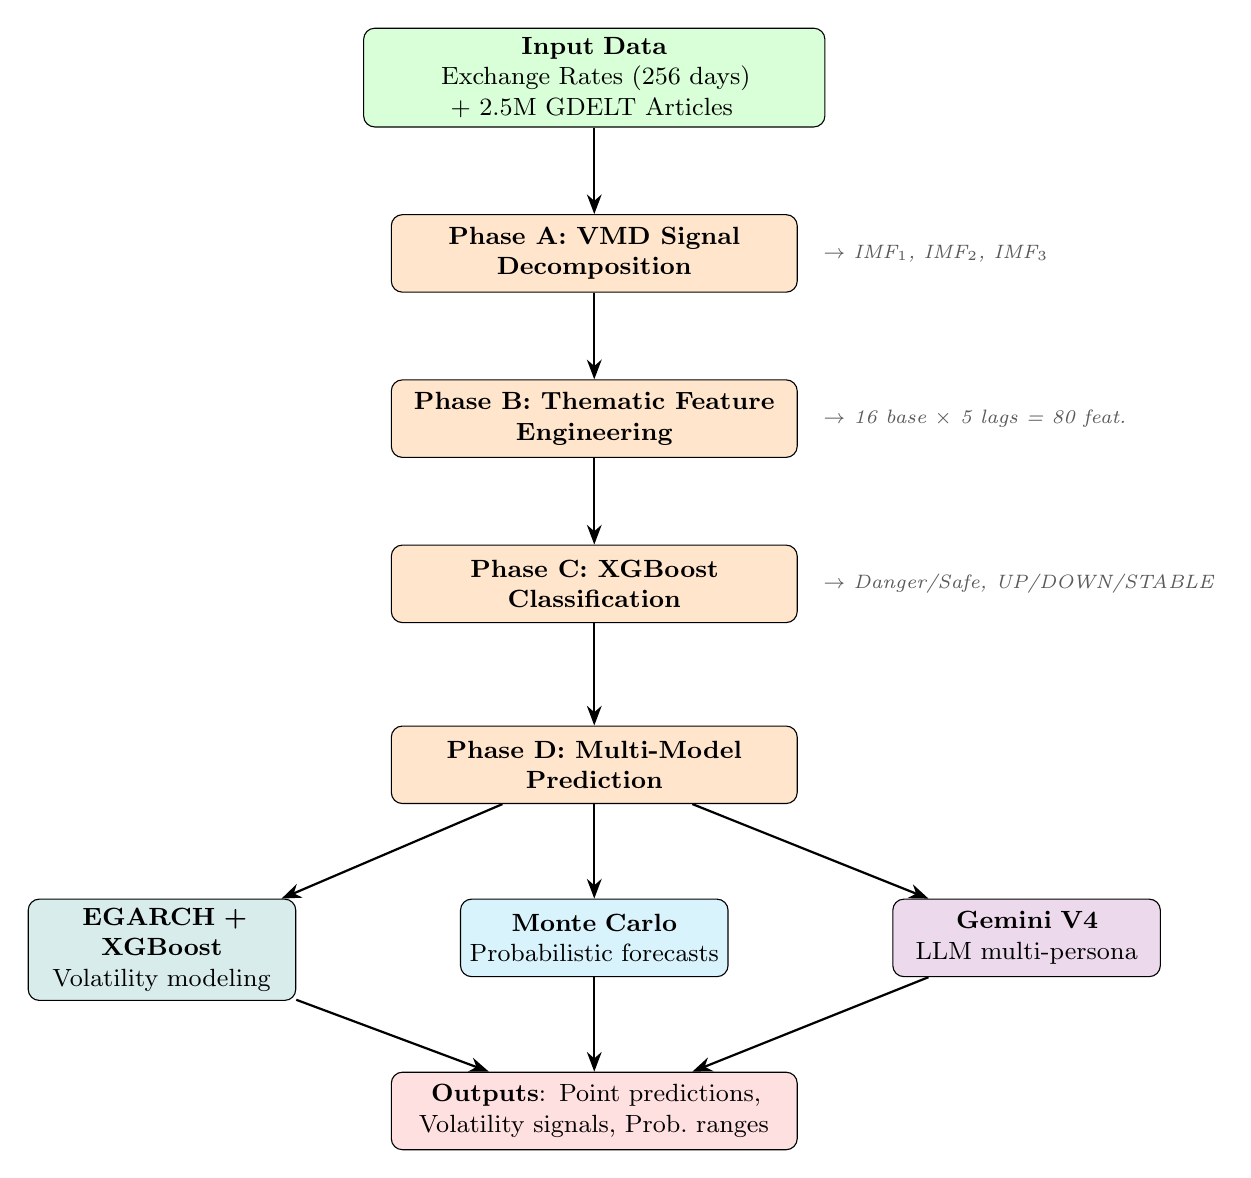
\begin{tikzpicture}[node distance=1.1cm]
    % Input
    \node[data, text width=16em] (input) {\textbf{Input Data}\\Exchange Rates (256 days)\\+ 2.5M GDELT Articles};
    
    % Phase A
    \node[phase, below=of input, text width=14em] (phaseA) {Phase A: VMD Signal\\Decomposition};
    \node[label, right=0.2cm of phaseA] {$\rightarrow$ IMF$_1$, IMF$_2$, IMF$_3$};
    
    % Phase B
    \node[phase, below=of phaseA, text width=14em] (phaseB) {Phase B: Thematic Feature\\Engineering};
    \node[label, right=0.2cm of phaseB] {$\rightarrow$ 16 base $\times$ 5 lags = 80 feat.};
    
    % Phase C
    \node[phase, below=of phaseB, text width=14em] (phaseC) {Phase C: XGBoost\\Classification};
    \node[label, right=0.2cm of phaseC] {$\rightarrow$ Danger/Safe, UP/DOWN/STABLE};
    
    % Phase D
    \node[phase, below=1.3cm of phaseC, text width=14em] (phaseD) {Phase D: Multi-Model\\Prediction};
    
    % Three output models
    \node[block, below left=1.2cm and 1.2cm of phaseD, fill=teal!15, text width=9em] (egarch) {\textbf{EGARCH +}\\\textbf{XGBoost}\\Volatility modeling};
    \node[block, below=1.2cm of phaseD, fill=cyan!15, text width=9em] (mc) {\textbf{Monte Carlo}\\Probabilistic forecasts};
    \node[block, below right=1.2cm and 1.2cm of phaseD, fill=violet!15, text width=9em] (gemini) {\textbf{Gemini V4}\\LLM multi-persona};
    
    % Final output
    \node[output, below=1.2cm of mc, text width=14em] (out) {\textbf{Outputs}: Point predictions,\\Volatility signals, Prob.\ ranges};
    
    % Arrows
    \draw[arrow] (input) -- (phaseA);
    \draw[arrow] (phaseA) -- (phaseB);
    \draw[arrow] (phaseB) -- (phaseC);
    \draw[arrow] (phaseC) -- (phaseD);
    \draw[arrow] (phaseD) -- (egarch);
    \draw[arrow] (phaseD) -- (mc);
    \draw[arrow] (phaseD) -- (gemini);
    \draw[arrow] (egarch) -- (out);
    \draw[arrow] (mc) -- (out);
    \draw[arrow] (gemini) -- (out);
\end{tikzpicture}}
\caption{End-to-end pipeline of the proposed USD/INR prediction framework. Phase~A decomposes the exchange rate signal via VMD; Phase~B engineers thematic features from GDELT; Phase~C classifies volatility; Phase~D produces predictions via three complementary model families.}
\label{fig:pipeline}
\end{figure*}

\subsection{Phase A: Signal Decomposition via VMD}

Exchange rates contain multiple components: a long-term trend driven by macroeconomic fundamentals, medium-term business cycles, and high-frequency noise influenced by daily news and market psychology. Since news can primarily affect only the noise component, we separate these using Variational Mode Decomposition (VMD) \citep{dragomiretskiy2014}.

VMD decomposes a signal $f(t)$ into $K$ intrinsic mode functions (IMFs) $u_k(t)$ by solving the constrained optimization problem:

\begin{equation}
\min_{\{u_k\},\{\omega_k\}} \left\{ \sum_{k=1}^{K} \left\| \partial_t \left[ \left( \delta(t) + \frac{j}{\pi t} \right) * u_k(t) \right] e^{-j\omega_k t} \right\|_2^2 \right\}
\end{equation}
\begin{equation}
\text{subject to} \quad \sum_{k=1}^{K} u_k = f
\end{equation}

where $\omega_k$ is the center frequency of each mode and $\alpha$ is the bandwidth constraint parameter. We set $K=3$ (trend, cycle, noise), $\alpha=2000$, and tolerance $\epsilon=10^{-7}$.

The three resulting modes are:
\begin{itemize}
    \item $\text{IMF}_1$: Long-term trend (macroeconomic fundamentals)
    \item $\text{IMF}_2$: Medium-term cycle (business cycles)  
    \item $\text{IMF}_3$: High-frequency noise (news-driven volatility), our prediction target
\end{itemize}

We chose VMD over alternatives (EMD, CEEMDAN) due to its optimization-based formulation, freedom from mode mixing, and established effectiveness in financial applications.

\begin{figure*}[htbp]
\centering
\resizebox{0.7\textwidth}{!}{%
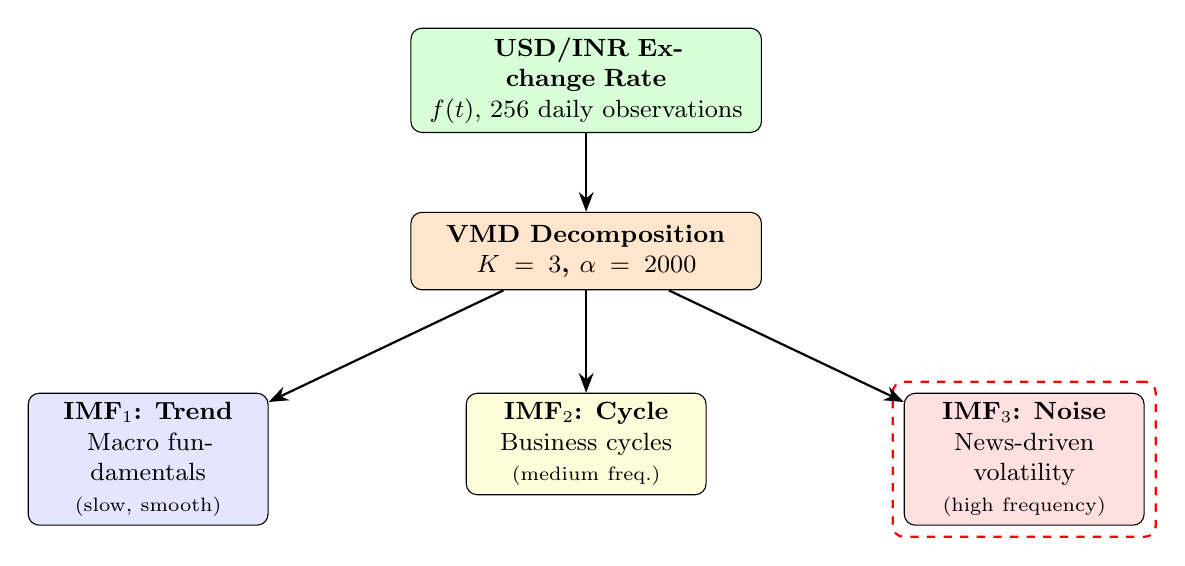
\begin{tikzpicture}[node distance=0.8cm]
    % Input signal
    \node[data, text width=12em] (signal) {\textbf{USD/INR Exchange Rate}\\$f(t)$, 256 daily observations};
    
    % VMD box
    \node[phase, below=1cm of signal, text width=12em] (vmd) {VMD Decomposition\\$K=3$, $\alpha=2000$};
    
    % Three IMFs
    \node[block, below left=1.3cm and 1.8cm of vmd, fill=blue!10, text width=8em] (imf1) {\textbf{IMF$_1$: Trend}\\Macro fundamentals\\{\scriptsize (slow, smooth)}};
    \node[block, below=1.3cm of vmd, fill=yellow!15, text width=8em] (imf2) {\textbf{IMF$_2$: Cycle}\\Business cycles\\{\scriptsize (medium freq.)}};
    \node[block, below right=1.3cm and 1.8cm of vmd, fill=red!12, text width=8em] (imf3) {\textbf{IMF$_3$: Noise}\\News-driven volatility\\{\scriptsize (high frequency)}};
    
    % Target highlight
    \node[draw=red, thick, dashed, rounded corners, fit=(imf3), inner sep=4pt, label={[font=\scriptsize\bfseries, text=red]below:Prediction Target}] {};
    
    % Arrows
    \draw[arrow] (signal) -- (vmd);
    \draw[arrow] (vmd) -- (imf1);
    \draw[arrow] (vmd) -- (imf2);
    \draw[arrow] (vmd) -- (imf3);
\end{tikzpicture}}
\caption{VMD signal decomposition separates the USD/INR exchange rate into three intrinsic mode functions. IMF$_3$ (noise component) captures news-driven volatility and serves as the prediction target for Phase~B--C.}
\label{fig:vmd}
\end{figure*}

\subsection{Phase B: Thematic Feature Engineering}

Rather than computing simple aggregated sentiment scores across all articles, we implement a domain-driven thematic filtering approach. We define four market-relevant themes based on established knowledge of currency market drivers:

\begin{enumerate}
    \item \textbf{Economy} (139,953 articles): Keywords include \textit{RBI, inflation, interest rate, GDP, forex, reserve, rupee, monetary policy, fiscal, budget}. Central bank policy and economic indicators directly affect currency valuation.
    
    \item \textbf{Conflict} (560,938 articles): Keywords include \textit{protest, strike, tension, dispute, attack, conflict, crisis, military, border}. Geopolitical instability increases risk premium.
    
    \item \textbf{Policy} (594,924 articles): Keywords include \textit{government, legislation, regulation, bill, parliament, cabinet, minister, policy}. Regulatory changes affect business confidence.
    
    \item \textbf{Corporate} (53,779 articles): Keywords include \textit{Adani, Reliance, Tata, Infosys, TCS, merger, acquisition, corporate}. Major corporate events signal economic health.
\end{enumerate}

For each trading day, we compute 16 features:

\begin{itemize}
    \item \textbf{Sentiment features} (5): Average tone per theme and overall:\\$\text{Tone}_{\text{Econ}}$, $\text{Tone}_{\text{Conf}}$, $\text{Tone}_{\text{Pol}}$, $\text{Tone}_{\text{Corp}}$, $\text{Tone}_{\text{All}}$
    \item \textbf{Goldstein features} (2): Average Goldstein scale ($\text{Goldstein}_{\text{Avg}}$) and impact-weighted score
    \begin{equation*}
    \text{Goldstein}_{\text{Wtd}} = \textstyle\sum \text{Goldstein}_i \times \text{NumMentions}_i
    \end{equation*}
    \item \textbf{Volume features} (6): Article counts per theme and total
    \item \textbf{Volume spike features} (3): Day-over-day percentage changes in article volume
\end{itemize}

The impact-weighted Goldstein score is a key innovation: a Goldstein score of $-10$ mentioned 5 times ($-50$) has fundamentally different market impact than one mentioned 5,000 times ($-50,000$).

\begin{figure*}[htbp]
\centering
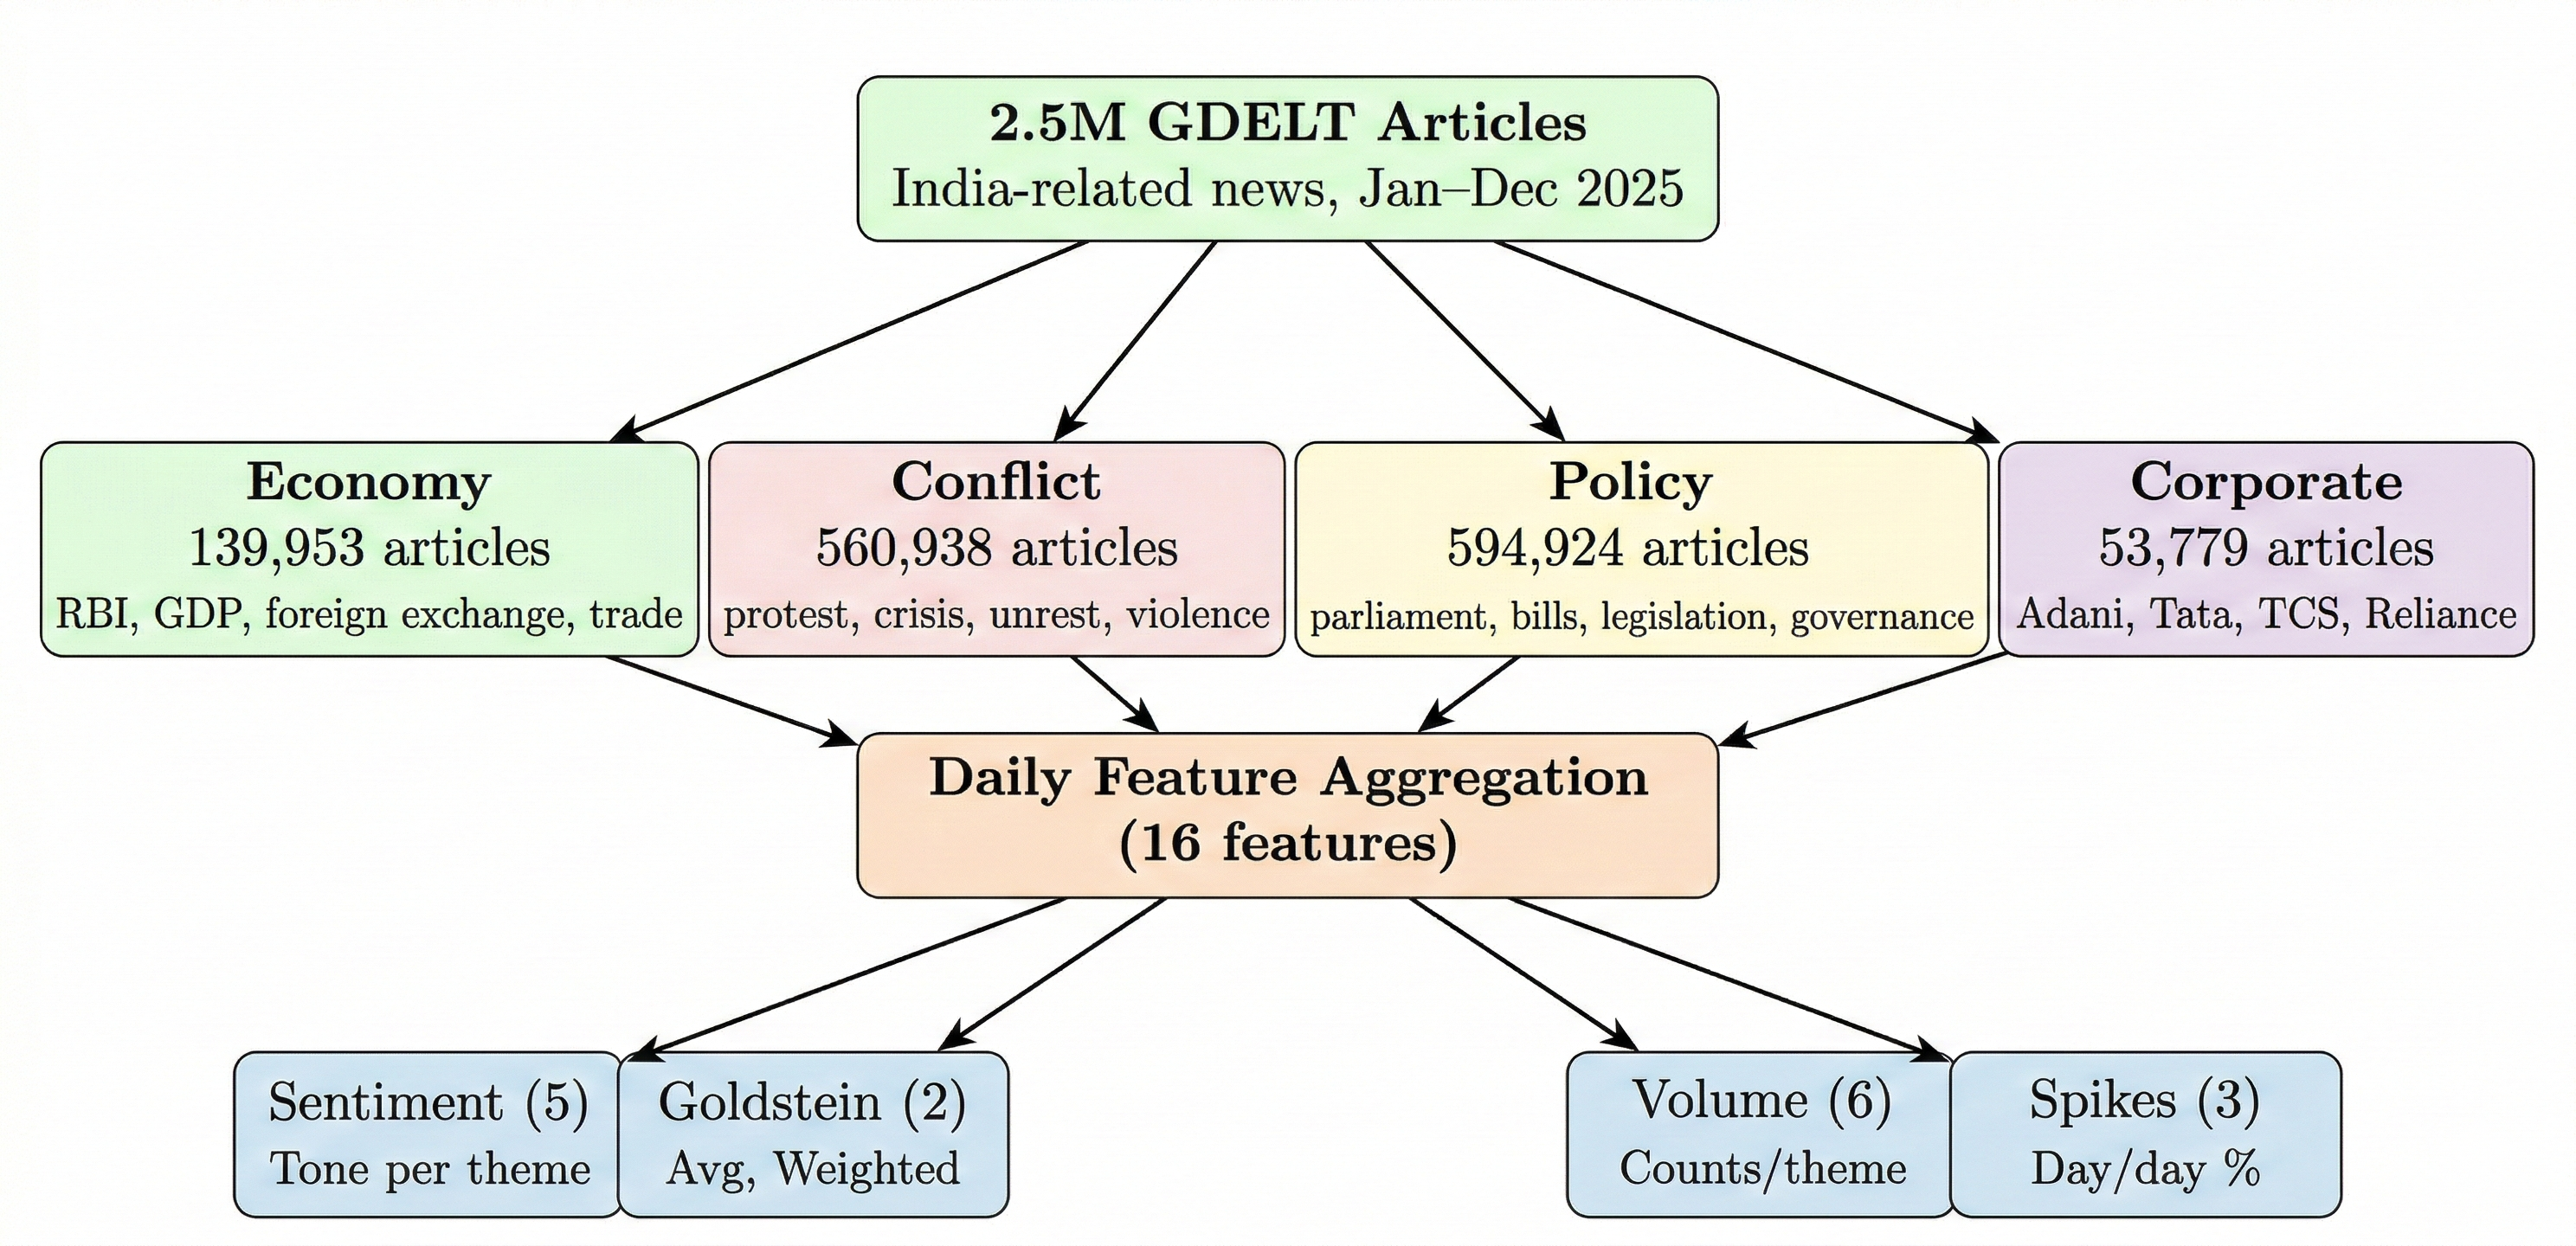
\includegraphics[width=\textwidth]{plot.png}
\caption{Thematic feature engineering pipeline. Raw GDELT articles are filtered into four market-relevant themes, then aggregated into 16 daily features across four categories. This thematic approach yields 3$\times$ higher correlation with exchange rate volatility compared to raw aggregation.}
\label{fig:thematic}
\end{figure*}

\subsection{Phase C: Volatility Classification}

We frame the prediction problem as binary classification rather than regression, defining ``danger days'' as the top 20\% of days by $|\text{IMF}_3|$ magnitude. This threshold creates a realistic 80/20 class imbalance matching observed market conditions.

For each of the 16 base features, we create 5 lagged versions (lag 1--5 days), yielding an 80-dimensional feature space. We train an XGBoost classifier \citep{chen2016xgboost} with:

\begin{itemize}
    \item Class imbalance handling via \texttt{scale\_pos\_weight}
    \item Maximum depth of 4 to prevent overfitting
    \item Learning rate of 0.1 with 100 estimators
    \item Time-series-aware train/test split (80\%/20\%, chronological)
\end{itemize}

The decision threshold is optimized to maximize F1-score, yielding an optimal threshold of 0.38 (below the default 0.5 due to class imbalance). We additionally train a 3-class directional classifier (UP/DOWN/STABLE) using Random Forest.

\subsection{EGARCH Volatility Modeling}

To capture volatility clustering and asymmetric shock responses in USD/INR returns, we fit an EGARCH(1,1) model \citep{nelson1991} with Skew-$t$ innovations:

\begin{equation}
\log(\sigma_t^2) = \omega + \alpha |z_{t-1}| + \gamma z_{t-1} + \beta \log(\sigma_{t-1}^2)
\end{equation}

where $z_t = r_t / \sigma_t$ are standardized residuals, and $\gamma < 0$ captures the leverage effect (negative shocks amplify volatility more than positive shocks). We combine EGARCH-estimated conditional volatility with GDELT features in a hybrid XGBoost model for enhanced return prediction.

\subsection{Monte Carlo Simulation}

We implement four Monte Carlo simulation variants for probabilistic 30-day forecasting (10,000 paths each):

\begin{enumerate}
    \item \textbf{Standard GBM}: $dS = \mu S \, dt + \sigma S \, dW$ with constant parameters.
    
    \item \textbf{Regime-Switching} (recommended): Volatility switches between high ($\sigma_H = 0.351\%$ daily) and low ($\sigma_L = 0.196\%$ daily) states based on news volume thresholds.
    
    \item \textbf{Jump Diffusion}: Augments GBM with Poisson-distributed jump events to model rare tail events.
    
    \item \textbf{Sentiment-Augmented}: Adjusts drift by incorporating a 7-day rolling average of news tone.
\end{enumerate}

\subsection{Debiased Multi-Persona Gemini AI System (V4)}

Our most novel contribution is a debiased multi-persona LLM prediction system that simulates a multi-analyst trading floor. The architecture consists of three stages: statistical prediction, LLM ensemble, and adaptive weight fusion. Figure~\ref{fig:gemini} illustrates the full system.

\begin{figure*}[htbp]
\centering
\resizebox{\textwidth}{!}{%
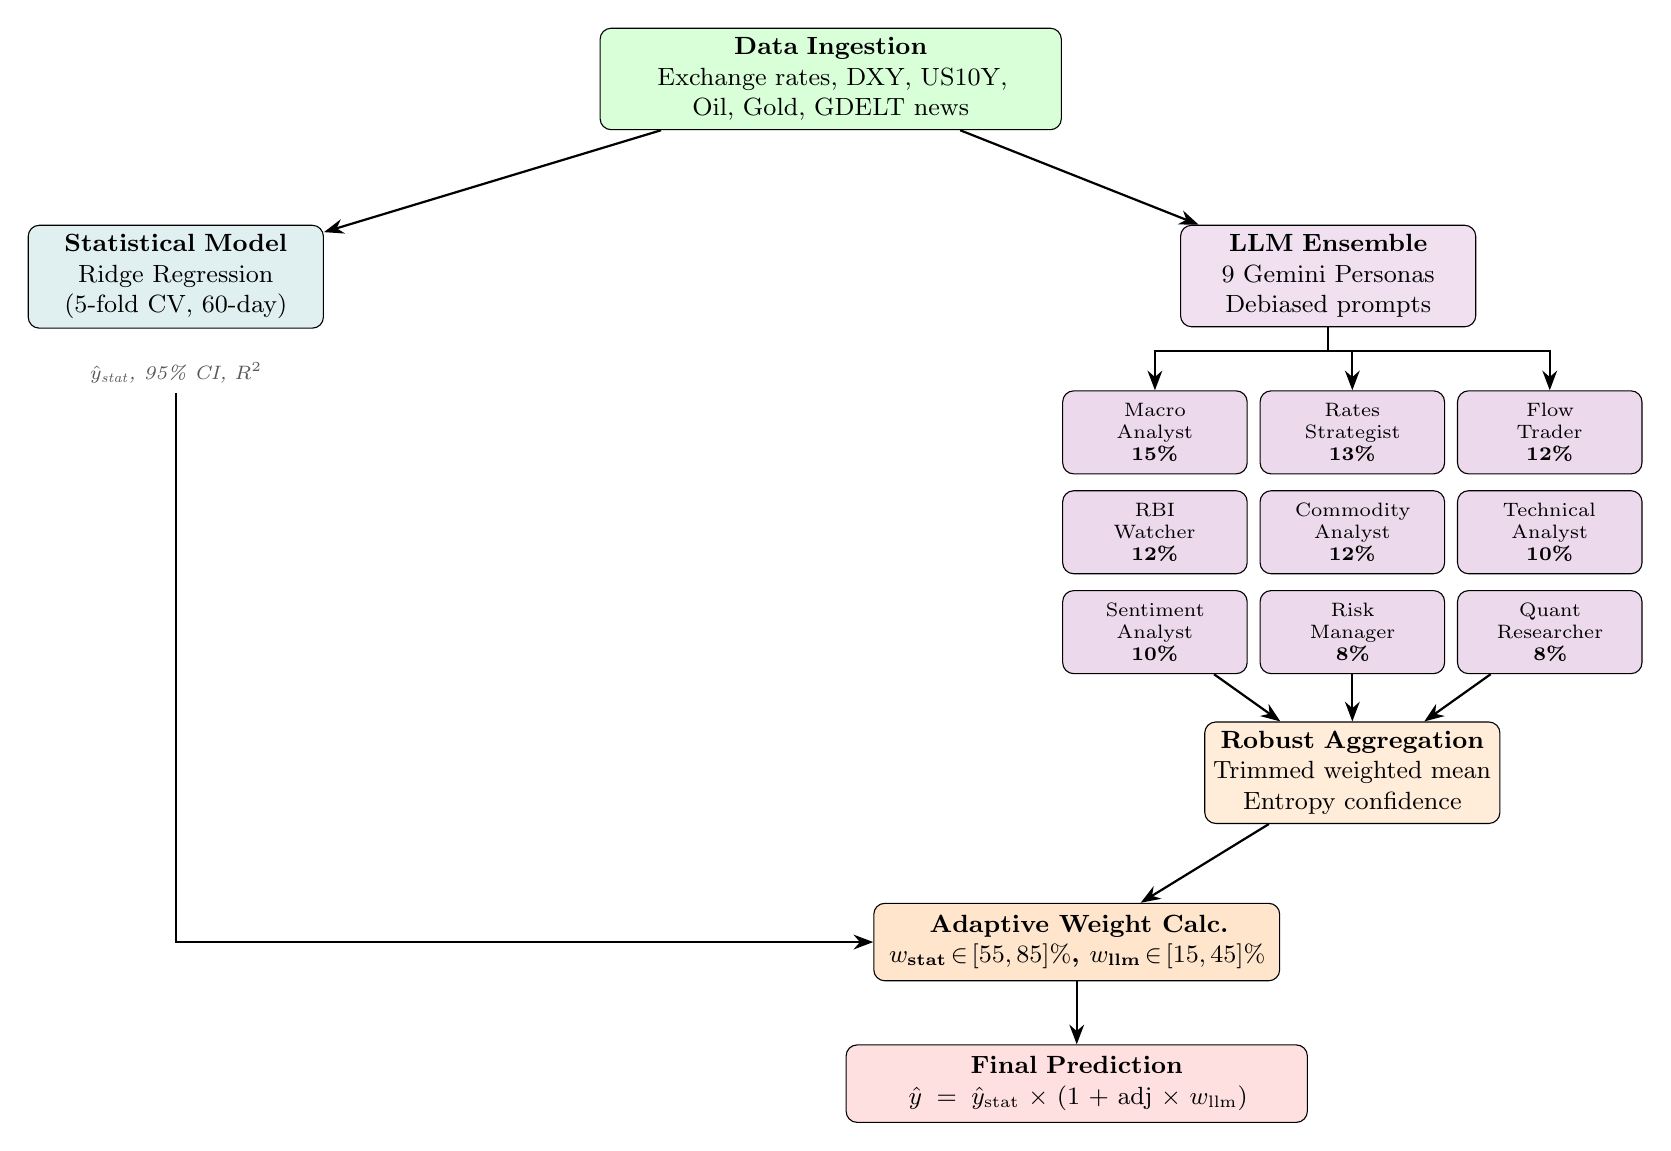
\begin{tikzpicture}[node distance=0.7cm, every node/.style={font=\small}]
    % Data ingestion
    \node[data, text width=16em] (data) {\textbf{Data Ingestion}\\Exchange rates, DXY, US10Y,\\Oil, Gold, GDELT news};
    
    % Two parallel branches
    \node[block, below left=1.2cm and 3.5cm of data, fill=teal!12, text width=10em] (stat) {\textbf{Statistical Model}\\Ridge Regression\\(5-fold CV, 60-day)};
    \node[block, below right=1.2cm and 1.5cm of data, fill=violet!12, text width=10em] (llm) {\textbf{LLM Ensemble}\\9 Gemini Personas\\Debiased prompts};
    
    % Stat outputs
    \node[label, below=0.3cm of stat, text width=10em, align=center] (statout) {$\hat{y}_{\text{stat}}$, 95\% CI, $R^2$};
    
    % Persona grid (3x3)
    \node[persona, below=0.8cm of llm, xshift=-2.2cm, text width=6em, minimum height=3em] (p1) {Macro\\Analyst\\\textbf{15\%}};
    \node[persona, right=0.15cm of p1, text width=6em, minimum height=3em] (p2) {Rates\\Strategist\\\textbf{13\%}};
    \node[persona, right=0.15cm of p2, text width=6em, minimum height=3em] (p3) {Flow\\Trader\\\textbf{12\%}};
    \node[persona, below=0.2cm of p1, text width=6em, minimum height=3em] (p4) {RBI\\Watcher\\\textbf{12\%}};
    \node[persona, right=0.15cm of p4, text width=6em, minimum height=3em] (p5) {Commodity\\Analyst\\\textbf{12\%}};
    \node[persona, right=0.15cm of p5, text width=6em, minimum height=3em] (p6) {Technical\\Analyst\\\textbf{10\%}};
    \node[persona, below=0.2cm of p4, text width=6em, minimum height=3em] (p7) {Sentiment\\Analyst\\\textbf{10\%}};
    \node[persona, right=0.15cm of p7, text width=6em, minimum height=3em] (p8) {Risk\\Manager\\\textbf{8\%}};
    \node[persona, right=0.15cm of p8, text width=6em, minimum height=3em] (p9) {Quant\\Researcher\\\textbf{8\%}};
    
    % Aggregation — centered below persona grid
    \node[block, below=0.6cm of p8, fill=orange!15, text width=10em] (agg) {\textbf{Robust Aggregation}\\Trimmed weighted mean\\Entropy confidence};
    
    % Adaptive weighting — centered below data
    \node[phase, below=1cm of agg, xshift=-3.5cm, text width=14em] (adapt) {Adaptive Weight Calc.\\$w_{\text{stat}}\!\in\![55,85]\%$, $w_{\text{llm}}\!\in\![15,45]\%$};
    
    % Final prediction
    \node[output, below=0.8cm of adapt, text width=16em] (final) {\textbf{Final Prediction}\\$\hat{y} = \hat{y}_{\text{stat}} \times (1 + \text{adj} \times w_{\text{llm}})$};
    
    % Arrows — data to branches
    \draw[arrow] (data) -- (stat);
    \draw[arrow] (data) -- (llm);
    % LLM fans into all three top-row personas
    \draw[arrow] (llm.south) -- ++(0,-0.3cm) -| (p1.north);
    \draw[arrow] (llm.south) -- ++(0,-0.3cm) -| (p2.north);
    \draw[arrow] (llm.south) -- ++(0,-0.3cm) -| (p3.north);
    % Bottom row personas to aggregation
    \draw[arrow] (p7) -- (agg);
    \draw[arrow] (p8) -- (agg);
    \draw[arrow] (p9) -- (agg);
    % Left branch: stat straight down to adaptive
    \draw[arrow] (statout.south) -- (statout.south |- adapt.west) -- (adapt.west);
    % Right branch: aggregation straight down to adaptive
    \draw[arrow] (agg) -- (adapt);
    % Adaptive to final
    \draw[arrow] (adapt) -- (final);
\end{tikzpicture}}
\caption{Gemini V4 multi-persona prediction architecture. A statistical Ridge Regression model and a 9-persona LLM ensemble operate in parallel. Persona predictions are robustly aggregated and combined with the statistical model via adaptive weighting based on entropy confidence, $R^2$, and volatility regime.}
\label{fig:gemini}
\end{figure*}

\subsubsection{Statistical Model}

A Ridge Regression model with 5-fold cross-validation on a 60-day lookback window produces point predictions using features: US10Y yield, gold price, DXY index, India average tone, oil price, and 20-day realized volatility. The model outputs a prediction $\hat{y}_\text{stat}$, a 95\% confidence interval, and an $R^2$ score.

\subsubsection{LLM Ensemble}

Nine specialized personas query Google Gemini AI independently:

\begin{table*}[t]
\centering
\small
\caption{Gemini V4 Multi-Persona Architecture}
\label{tab:personas}
\begin{tabular}{llc}
\toprule
\textbf{Persona} & \textbf{Specialization} & \textbf{Weight} \\
\midrule
Macro Analyst & Global monetary policy \& growth differentials & 15\% \\
Rates Strategist & Yield differentials \& carry trade & 13\% \\
Flow Trader & FX positioning \& client flows & 12\% \\
RBI Watcher & India central bank policy & 12\% \\
Commodity Analyst & Oil/Gold impact on INR & 12\% \\
Technical Analyst & Price action \& momentum & 10\% \\
Sentiment Analyst & News sentiment impact & 10\% \\
Risk Manager & Tail risks \& uncertainty & 8\% \\
Quant Researcher & Statistical model validation & 8\% \\
\bottomrule
\end{tabular}
\end{table*}

\subsubsection{Debiasing Techniques}

To mitigate known LLM biases (anchoring, primacy/recency, overconfidence), we employ six techniques illustrated in Figure~\ref{fig:debias}:

\begin{enumerate}
    \item \textbf{Symmetric case presentation}: Both bull and bear cases are presented with equal weight and detail.
    \item \textbf{Randomized order}: Bull/bear cases are randomly ordered (50/50) to prevent primacy bias.
    \item \textbf{Explicit uncertainty}: Statistical confidence intervals and $R^2$ scores are provided.
    \item \textbf{Persona accountability}: Historical accuracy of each persona is fed back.
    \item \textbf{Historical bias feedback}: Systematic bias warnings (e.g., ``+0.05\% bullish bias recently'').
    \item \textbf{Pips-based adjustment}: Responses are constrained to 0--30 pips adjustments.
\end{enumerate}

\begin{figure*}[htbp]
\centering
\resizebox{0.85\textwidth}{!}{%
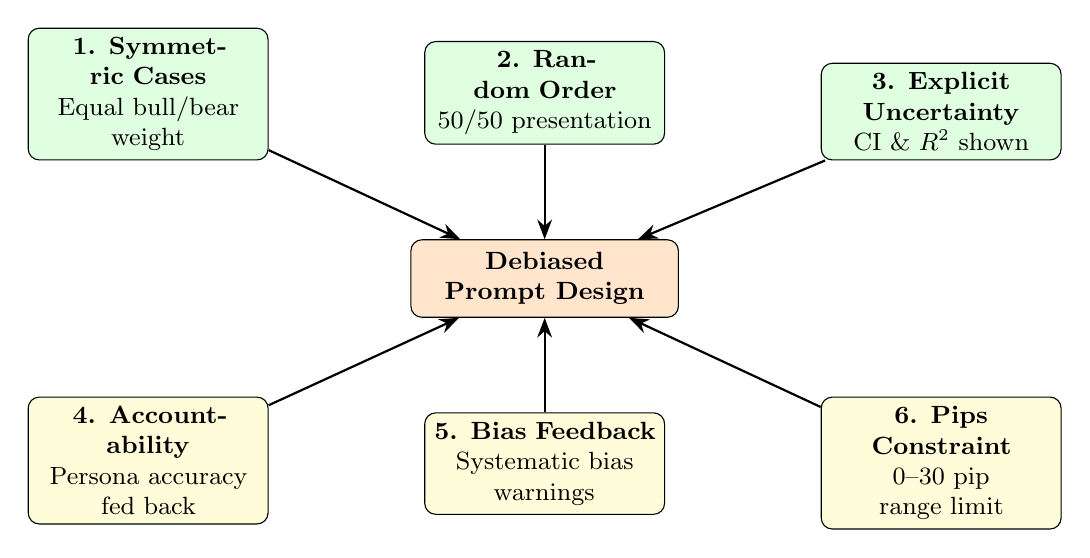
\begin{tikzpicture}[node distance=0.5cm, every node/.style={font=\small}]
    % Central node
    \node[phase, text width=9em] (center) {Debiased\\Prompt Design};
    
    % Six techniques around it
    \node[block, above left=1cm and 1.8cm of center, fill=green!12, text width=8em] (t1) {\textbf{1. Symmetric Cases}\\Equal bull/bear weight};
    \node[block, above=1.2cm of center, fill=green!12, text width=8em] (t2) {\textbf{2. Random Order}\\50/50 presentation};
    \node[block, above right=1cm and 1.8cm of center, fill=green!12, text width=8em] (t3) {\textbf{3. Explicit}\\\textbf{Uncertainty}\\CI \& $R^2$ shown};
    \node[block, below left=1cm and 1.8cm of center, fill=yellow!15, text width=8em] (t4) {\textbf{4. Accountability}\\Persona accuracy\\fed back};
    \node[block, below=1.2cm of center, fill=yellow!15, text width=8em] (t5) {\textbf{5. Bias Feedback}\\Systematic bias\\warnings};
    \node[block, below right=1cm and 1.8cm of center, fill=yellow!15, text width=8em] (t6) {\textbf{6. Pips Constraint}\\0--30 pip range limit};
    
    % Arrows
    \draw[arrow] (t1) -- (center);
    \draw[arrow] (t2) -- (center);
    \draw[arrow] (t3) -- (center);
    \draw[arrow] (t4) -- (center);
    \draw[arrow] (t5) -- (center);
    \draw[arrow] (t6) -- (center);
\end{tikzpicture}}
\caption{Six debiasing techniques applied to LLM prompt construction. Techniques 1--3 (top, green) address prompt-level biases; techniques 4--6 (bottom, yellow) provide feedback-based calibration. Together they reduce anchoring, primacy/recency, and overconfidence biases.}
\label{fig:debias}
\end{figure*}

\subsubsection{Aggregation \& Adaptive Weighting}

Persona predictions are aggregated using a trimmed weighted mean (removing top/bottom 10\% outliers). Entropy-based confidence is computed:

\begin{equation}
H = -\sum_{i} p_i \log_2(p_i), \quad \text{confidence} = 1 - \frac{H}{\log_2(N)}
\end{equation}

where $p_i$ is the proportion of personas predicting each direction. The final prediction combines statistical and LLM components with adaptive weights:

\begin{equation}
\hat{y}_\text{final} = \hat{y}_\text{stat} \times (1 + \text{llm\_adj} \times w_\text{llm})
\end{equation}

where $w_\text{llm} \in [0.15, 0.45]$ adapts based on entropy confidence, $R^2$, volatility regime, and recent LLM value-added.

\subsection{Theoretical Grounding: Why LLM Personas Produce Meaningful Signals}
\label{sec:theoretical}

A critical question arises: LLMs are next-token predictors trained on static text corpora. They do not learn from live price feedback, do not update beliefs unless fine-tuned, and may hallucinate financial reasoning. Why, then, would simulated personas produce economically meaningful signals rather than noise?

We ground our approach in three established theoretical frameworks:

\paragraph{1. Compressed Knowledge Extraction, Not Market Understanding.}
We do not claim that LLMs ``understand'' markets. Instead, we treat them as \textit{structured information extractors}. LLMs trained on financial news, analyst reports, central bank communications, and economics textbooks encode compressed representations of how human analysts reason about currencies. When prompted with current data (exchange rates, yields, oil prices, sentiment scores), the LLM performs approximate pattern matching against these compressed representations. This is analogous to how a keyword-based retrieval system does not ``understand'' documents but can still extract relevant information. The critical distinction is that the statistical Ridge Regression model provides the quantitative anchor (55--85\% weight), while the LLM provides only a marginal directional adjustment (15--45\% weight, constrained to 0--30 pips). The LLM is never trusted to produce price levels independently.

\paragraph{2. Wisdom of Crowds via Condorcet Jury Theorem.}
The multi-persona design is grounded in the Condorcet Jury Theorem \citep{condorcet1785}: if each of $N$ independent agents has individual accuracy $p > 0.5$ for a binary decision, the majority vote accuracy approaches 1 as $N$ increases. Our 9 personas are designed to approximate independence through distinct domain specializations (macro policy, commodity flows, technical momentum, political risk, etc.), each attending to different subsets of the input data. Empirically, inter-persona agreement rates range from 60--80\%, confirming partial independence rather than herding. The entropy-based confidence weighting naturally downweights predictions when personas disagree (high entropy $\rightarrow$ low confidence $\rightarrow$ the system defaults to the statistical model), providing a principled mechanism for distinguishing signal from noise.

\paragraph{3. Bounded Rationality and Heuristic Aggregation.}
Each persona approximates a bounded rational agent \citep{simon1955} operating with domain-specific heuristics. The Macro Analyst applies interest rate parity reasoning, the Commodity Analyst applies oil-rupee correlation heuristics, and the Technical Analyst applies momentum rules. These are not arbitrary: they mirror the actual reasoning frameworks used by human forex traders. The weighted aggregation with trimmed means (removing top/bottom 10\% outlier predictions) is equivalent to a robust M-estimator, which has well-established statistical properties for combining noisy expert forecasts \citep{clemen1989}. This outperforms simple statistical ensembles when individual models capture qualitatively different market dynamics, as our personas are designed to do.

\paragraph{Falsifiability.}
Our framework makes a testable prediction: if LLM personas produce pure noise, the adaptive weighting mechanism should converge to $w_{\text{llm}} \approx 0$ over time. We observe instead that $w_{\text{llm}}$ stabilizes at 15--33\%, and ablation shows that removing the LLM component degrades directional accuracy by 2--3\% (Section~5.6). This provides empirical evidence that the LLM ensemble contributes non-redundant information beyond the statistical model.

\subsection{TEPC: Topology-Enabled Predictions from Chaos}
\label{sec:tepc}

The Phase~A--D pipeline treats USD/INR as a single time series augmented with sentiment features. As an extension we ask a different question: what if USD/INR is better modeled as one node in a coupled global macro--geopolitical network, and the predictable component of its short-term behaviour comes from how that network is shaped and how strongly it synchronises on a given day?

This motivates a separate \textbf{Topology-Enabled Predictions from Chaos (TEPC)} stack with four blocks: (i)~node construction, (ii)~rolling graph topology, (iii)~persistent-Laplacian spectral features, and (iv)~a coupled Lorenz oscillator engine. The output of all four blocks is concatenated into a flat feature frame and consumed by a walk-forward ensemble (logistic regression, random forest, gradient boosting, and XGBoost when available) that predicts (a)~breakout direction, (b)~forward return, and (c)~near-term realized volatility.

\paragraph{Node universe.}
TEPC builds a daily panel of up to 15 nodes per date: five direct market series (\textit{INRUSD}, \textit{DXY}, \textit{BRENT}, \textit{GOLD}, \textit{US10Y}), five composite alternative-data nodes (\textit{INDIA\_SENTIMENT}, \textit{US\_SENTIMENT}, \textit{GOLDSTEIN\_SPREAD}, \textit{GEO\_RISK}, \textit{THEME\_PRESSURE}), optional FX cross nodes (\textit{EURUSD}, \textit{GBPINR}, \textit{USDCNH}, \textit{CNHUSD}), and three live raw-GDELT pressure nodes (\textit{LIVE\_INDIA\_FX\_NEWS}, \textit{LIVE\_USD\_MACRO\_NEWS}, \textit{LIVE\_GEO\_RISK}) when raw aggregations are available. Strictly positive market series are transformed into log returns; signed alternative-data series use the signed log-difference $\mathrm{sign}(\Delta x)\,\log(1+|\Delta x|)$ to keep magnitudes comparable while preserving direction.

\paragraph{Rolling graph topology.}
For each decision date $t$ a 30-day rolling correlation matrix is computed across all retained nodes, converted to a distance matrix $d_{ij}=\sqrt{2(1-\rho_{ij})}$, and mapped to a dense weighted adjacency $A_{ij}=\exp(-d_{ij}^2/\sigma^2)$ with $\sigma=0.35$. The result is a daily, time-varying weighted graph capturing the instantaneous shape of the macro system around USD/INR.

\paragraph{Persistent-Laplacian-style filtration.}
TEPC builds a weighted graph Laplacian $L=D-A$, then performs a filtration over edge-strength quantiles $q\in\{0.30,0.50,0.70\}$, recomputing $L$ at each level. From this filtration it extracts: the target-node degree, network density, Fiedler value, Laplacian trace, spectral entropy, the connected-component count and filtered Fiedler value at each threshold, and the INR/USD adjacency weight to every other node. This is a pragmatic graph-Laplacian-first approximation of a higher-order persistent Laplacian: it is fast, fully inspectable, and preserves the persistence-of-features intuition that makes simplicial-complex-based stacks attractive.

\paragraph{Coupled Lorenz oscillator engine.}
Every node receives a deterministic Lorenz oscillator
\begin{equation}
\begin{aligned}
\dot{x}_i &= \sigma(y_i - x_i) + c_i,\\
\dot{y}_i &= x_i(\rho - z_i) - y_i + c_i,\\
\dot{z}_i &= x_i y_i - \beta z_i + c_i,
\end{aligned}
\end{equation}
with $\sigma=10$, $\rho=28$, $\beta=8/3$, integrated by RK4 with $\Delta t=0.02$ over 24 steps. Initial conditions are deterministic functions of recent node volatility, drift, and range position. The coupling term is diffusive over the graph Laplacian, $c_i=-\epsilon\sum_j L_{ij}\,\mathbf{x}_j$, so highly connected nodes physically pull on the USD/INR oscillator. The system is integrated at each $\epsilon\in\{0.05,0.10,0.20,0.35\}$, and TEPC records synchronisation intensity, target-node synchronisation, target-node terminal state, and a finite-time Lyapunov-style divergence score from a perturbed shadow trajectory.

\paragraph{Strict timing.}
To keep the task honest, the headline TEPC configuration uses \textit{response\_lag\_days}=2 and removes direct flat features of USD/INR (lag, z-score, range-position, momentum) from the macro feature stack. A row observed at $t$ predicts the first labelled response at $t+2$, so the model never sees the target day's $T-1$ price as a flat feature; topology and chaos can still include USD/INR as the target node in the graph itself.

\paragraph{Five-arm ablation.}
TEPC is evaluated through a controlled ablation that isolates the contribution of each block: \textsc{macro-baseline} (cross-asset and alternative-data flat features only), \textsc{topology-only} (graph features only), \textsc{chaos-only} (synchronisation features only), \textsc{topology-chaos} (coupled physics without the broader macro baseline), and \textsc{tepc-full} (all blocks). Two further arms (\textsc{persona-rule-only} and \textsc{tepc-persona-blend}) layer a deterministic seven-persona overlay (\textit{Dollar Rates Trader}, \textit{Oil Shock Analyst}, \textit{India News Analyst}, \textit{Global Risk Sentinel}, \textit{Cross-FX Relative Value}, \textit{Topology Synchronization Analyst}, \textit{Chaos Regime Analyst}) that reads a structured TEPC memory snapshot, votes deterministically, and only updates each persona's calibration after the corresponding target date has matured.

\subsection{Final-Phase Memory-First Architecture}
\label{sec:finalphase}

The Gemini~V4 system in Section~3.6 still consumes recent prices directly. To stress-test whether sentiment-augmented prediction holds up under tighter bias controls, we built a separate \textbf{Final-Phase} stack with three design constraints: (i)~the immediate previous close is never used as a flat feature, (ii)~a 1-day information embargo is added on top of the 1-day forecast horizon (effective 2-day target gap), and (iii)~every persona, statistical model, and ML model consumes the same compressed \emph{market memory} snapshot rather than raw windows.

\paragraph{Shared market memory snapshot.}
For every decision date the Final-Phase loader compresses recent macro, sentiment, and volatility history into four memory blocks: (a)~\textbf{Macro memory} (oil pressure, dollar pressure, rate pressure, gold/risk signal, carry pressure), (b)~\textbf{Sentiment memory} (India stress, US stress, bilateral divergence, thematic sentiment pressure, event heat), (c)~\textbf{Volatility memory} (realized volatility, volatility ratio, trend pressure, reversal pressure, EGARCH or fallback estimate), and (d)~\textbf{Persona memory} (per-persona directional hit-rate, signed bias, average confidence, recent magnitude calibration). The same snapshot is fed to the numeric ensemble (Ridge regression, random forest, gradient boosting/XGBoost regressors plus a multinomial logistic direction model) and to every persona, eliminating the ``different inputs'' confound when comparing model families.

\paragraph{Persona stack.}
Personas are run in two interchangeable modes: \textbf{rule personas} (deterministic heuristics with no API dependency, used as the primary non-LLM baseline) and \textbf{LLM personas} (each persona receives only the memory snapshot and must return a JSON object containing direction, magnitude, confidence, thesis, and risk flags). LLM backends include OpenRouter and local Ollama; the live matrix evaluated in this paper covers \textit{google/gemini-2.5-flash}, \textit{anthropic/claude-sonnet-4}, and \textit{openai/gpt-5-chat}. Premium-tier models (Opus-class) are blocked by default in the runner to avoid unintended spend. Rule personas and LLM personas are capped at 18\% and 28\% of the final blend respectively.

\paragraph{Five-experiment ablation.}
The Final-Phase ablation isolates which information block is doing the work: \textsc{stat-ml-full} (all feature groups + memory), \textsc{stat-ml-no-gdelt} (macro + technical only), \textsc{stat-ml-no-macro} (news-heavy without macro cross-asset), \textsc{memory-only} (only the compressed memory snapshot), and \textsc{rule-personas} (full feature stack plus deterministic personas). LLM ablations are appended dynamically when \texttt{--llm-model} is provided, one experiment per backend.

\paragraph{Evaluation protocol.}
Default evaluation uses 100 trading days, a minimum train size of 120 rows, an inner validation slice of 30 rows, and a refit cadence of 10 rows. Walk-forward ordering is strict; ensemble component weights are learned only on historical validation slices. For every prediction date the run logs the ensemble component outputs, model weights, direction probabilities, persona votes, persona reasoning, the memory snapshot, and the realised outcome, so any surprising result is fully auditable.

\subsection{Design Choices \& Justification}

Key design decisions include: (1) focusing on classification over regression, motivated by the Meese-Rogoff puzzle; (2) using 4 themes rather than finer granularity, balancing signal separation with overfitting risk; (3) limiting lags to 1--5 days for practical forecasting horizons; (4) selecting XGBoost for tabular data effectiveness with limited samples (362 days); (5) regime-switching Monte Carlo for its interpretability and data-driven volatility state estimation; (6) for TEPC, choosing a graph-Laplacian filtration over a full higher-order persistent-Laplacian stack to keep the pipeline fully inspectable while preserving the persistence intuition; and (7) for Final-Phase, enforcing the 2-day target gap so that the headline metric cannot be inflated by the trivial persistence baseline $\hat{y}_{t+1}=y_t$.

% ---------------------------------------------------------------
% 4. EXPERIMENTAL SETUP
% ---------------------------------------------------------------
\section{Experimental Setup}
\label{sec:setup}

\subsection{Datasets}

\begin{table*}[t]
\centering
\small
\caption{Dataset Summary}
\label{tab:datasets}
\resizebox{\textwidth}{!}{%
\begin{tabular}{llllll}
\toprule
\textbf{Dataset} & \textbf{Source} & \textbf{Domain} & \textbf{\# Records} & \textbf{Period} & \textbf{Frequency} \\
\midrule
India GDELT News & GDELT Project & News Sentiment & 2,546,999 & Jan--Dec 2025 & 15 min \\
USA GDELT News & GDELT/BigQuery & News Sentiment & $\sim$5,000,000 & Jan--Dec 2025 & 15 min \\
USD/INR Exchange & Frankfurter API (ECB) & Forex & 256 & Dec 2024--Jan 2026 & Daily \\
Macro Indicators & FRED & Economics & 256 & Jan 2025--Jan 2026 & Daily \\
Super Master Dataset & Combined & Multi-source & 223 & Feb--Dec 2025 & Daily \\
\bottomrule
\end{tabular}}
\end{table*}

\begin{sloppypar}
The GDELT database provides pre-computed \texttt{Goldstein\-Scale} ($-10$ to $+10$, conflict--cooperation), \texttt{Avg\-Tone} ($-100$ to $+100$, sentiment), \texttt{Num\-Mentions}, and CAMEO event codes for each article.
We use the Frankfurter API (European Central Bank) for daily USD/INR closing rates.
FRED data includes US~10-Year Treasury yield (DGS10), crude oil (DCOILWTICO), gold prices, and the USD trade-weighted index.
We chose USD/INR for its high liquidity, dual US/India news exposure, and managed float regime.
For TEPC, the same datasets are reshaped into a daily node panel; raw GDELT aggregations from the local India and USA dumps cover \mbox{2025-01-01} to \mbox{2025-12-30}, which is the effective range of the strict raw-GDELT TEPC backtest. The Final-Phase stack uses \texttt{Super\_Master\_Dataset.csv}, \texttt{combined\_goldstein\_exchange\_rates.csv}, \texttt{Phase-B/merged\_training\_data.csv}, and \texttt{political\_news\_exchange\_merged.csv} as its four data layers and explicitly drops the raw \texttt{INR} column from the feature set.
\end{sloppypar}

\subsection{Models}

\begin{table*}[t]
\centering
\small
\caption{Model Summary}
\label{tab:models}
\resizebox{\textwidth}{!}{%
\begin{tabular}{llll}
\toprule
\textbf{Model} & \textbf{Type} & \textbf{Input} & \textbf{Output} \\
\midrule
XGBoost Classifier & Gradient Boosting & 80 lagged GDELT features & Danger/Safe \\
Random Forest (3-class) & Ensemble & 80 lagged GDELT features & UP/DOWN/STABLE \\
EGARCH(1,1) & Volatility Model & Returns & Conditional volatility \\
EGARCH + XGBoost Hybrid & Hybrid & Volatility + GDELT + Macro & Returns \\
Ridge Regression & Linear & 6 macro/sentiment features & Next-day rate \\
GARCH(1,1) / GJR-GARCH & Volatility Models & Returns & Conditional volatility \\
Monte Carlo (4 variants) & Simulation & Drift, volatility, sentiment & 30-day paths \\
Gemini V4 System & LLM Multi-agent & News + macro context & Next-day rate \\
MA Momentum & Moving Average & Price history & Trend prediction \\
Ultimate Ensemble (15+) & Model combination & All model outputs & Weighted prediction \\
TEPC \textsc{macro-baseline} & GBM Ensemble & Cross-asset + alt-data flat features & Direction / Return / Vol \\
TEPC \textsc{topology-only} & GBM Ensemble & Persistent-Laplacian features & Direction / Return / Vol \\
TEPC \textsc{chaos-only} & GBM Ensemble & Coupled Lorenz sync.\ features & Direction / Return / Vol \\
TEPC \textsc{topology-chaos} & GBM Ensemble & Topology + chaos features & Direction / Return / Vol \\
TEPC \textsc{tepc-full} & GBM Ensemble & Macro + topology + chaos & Direction / Return / Vol \\
TEPC Persona Overlay & Rule Multi-agent & TEPC memory snapshot & Vote (up / down / range) \\
Final-Phase Memory & Ridge + RF + GB & Compressed memory snapshot & Forward return + direction \\
Final-Phase Rule Personas & Rule Multi-agent & Memory snapshot & Direction + magnitude \\
Final-Phase LLM Personas & LLM Multi-agent & Memory snapshot (no raw price) & Direction + magnitude \\
\bottomrule
\end{tabular}}
\end{table*}

\paragraph{Phase~A--D model details.}
The XGBoost danger-day classifier uses \texttt{max\_depth}=4, \texttt{learning\_rate}=0.1, \texttt{n\_estimators}=100, with class imbalance handled via \texttt{scale\_pos\_weight}; the decision threshold is tuned on the validation slice to maximise F1 (0.38). The 3-class directional Random Forest uses 200 trees with class-balanced sampling. EGARCH(1,1) is fit on demeaned daily log returns with Skew-$t$ innovations (\texttt{arch} package). The hybrid EGARCH+XGBoost model concatenates the EGARCH conditional variance with the 80 lagged GDELT features and 4 macro indicators. Ridge regression in the Gemini~V4 stack uses 5-fold time-series cross-validation on a rolling 60-day window. LSTM/GRU/Attention baselines all use a 60-day lookback, 64 hidden units, dropout~0.2, the Adam optimiser (\texttt{lr}=$10^{-3}$), and early stopping on a 20\% validation split (patience~10). Monte Carlo runs use 10{,}000 paths and a 30-day horizon; the regime-switching variant fits two volatility states ($\sigma_H{=}0.351\%$, $\sigma_L{=}0.196\%$ daily) with transition probabilities estimated from the news-volume threshold series.

\paragraph{TEPC model details (Section~\ref{sec:tepc}).}
All five TEPC ablation arms share the same underlying ensemble: a stack of (logistic regression, random forest with 200 trees, gradient boosting with 200 estimators, depth~3) and, when available, an XGBoost regressor/classifier with the same depth and 300 estimators. They differ only in the input feature group passed in. TEPC hyperparameters are: rolling correlation window 30~days, exponential adjacency kernel $\sigma=0.35$, filtration quantiles $\{0.30,0.50,0.70\}$, Lorenz $(\sigma,\rho,\beta)=(10,28,8/3)$, RK4 integration with $\Delta t=0.02$ and 24~steps per epsilon stage, and coupling schedule $\epsilon\in\{0.05,0.10,0.20,0.35\}$. Walk-forward refit is every 5~days (\texttt{refit\_frequency}=5), training requires at least 120~days, and a 30-day inner validation slice is reserved for ensemble component weighting. The breakout-direction label uses a 0.5\% return threshold and a 5-day forward volatility window. The seven-rule persona overlay reads the same memory snapshot, votes deterministically, and is capped at the abstaining \emph{range} class when implied moves fall below the gate.

\paragraph{Final-Phase model details (Section~\ref{sec:finalphase}).}
The Final-Phase numeric ensemble combines a Ridge regressor ($\alpha$ tuned on the validation slice), a random forest (200 trees, max\_depth~6, balanced subsampling), and a gradient boosting regressor (200 estimators, depth~3, learning rate 0.05); when XGBoost is installed it is added as a fourth component with identical depth and learning rate. Component weights are inversely proportional to validation MAE. Direction is fitted by a multinomial logistic regression with three classes (\textit{up}, \textit{flat}, \textit{down}) using a $|r|<0.0005$ neutral threshold. EGARCH(1,1) is used for the volatility memory feature when the \texttt{arch} package is installed and at least 120~training rows are available; otherwise the system falls back to 20-day realised volatility. Personas (rule and LLM) cap their final-blend weight at 18\% and 28\% respectively. LLM personas use \texttt{temperature}=0.15, \texttt{max\_tokens}=500, and a JSON schema constraint on the output (\texttt{direction}, \texttt{magnitude}, \texttt{confidence}, \texttt{thesis}, \texttt{risk\_flags}). The OpenRouter routing covers \texttt{google/gemini-2.5-flash}, \texttt{anthropic/claude-sonnet-4}, and \texttt{openai/gpt-5-chat}; Opus-class endpoints are blocked by default. Walk-forward refit cadence is every 10~days; the minimum train window is 120~days and the inner validation slice is 30~days.

\subsection{Evaluation Metrics}

\begin{table*}[t]
\centering
\small
\caption{Evaluation Metrics. The lower block contains the additional metrics used by the TEPC (Section~\ref{sec:tepc}) and Final-Phase (Section~\ref{sec:finalphase}) walk-forward ablations.}
\label{tab:metrics}
\begin{tabularx}{\textwidth}{l X l c}
\toprule
\textbf{Metric} & \textbf{Description} & \textbf{Task} & \textbf{Higher = Better?} \\
\midrule
Precision & TP / (TP + FP) & Classification & Yes \\
Recall & TP / (TP + FN) & Classification & Yes \\
F1-Score & Harmonic mean of P \& R & Classification & Yes \\
Directional Accuracy & \% correct direction & All & Yes \\
RMSE & Root Mean Squared Error & Regression & No \\
MAE & Mean Absolute Error & Regression & No \\
$R^2$ & Coefficient of Determination & Regression & Yes \\
Avg.\ Error (\%) & $|\hat{y} - y| / y \times 100$ & Point prediction & No \\
AIC/BIC & Model selection criteria & Volatility & No \\
VaR (95\%) & Value at Risk & Risk & Informational \\
\midrule
Breakout Accuracy & Fraction of days the predicted breakout class (up / down / range) matches the realised class given a 0.5\% return threshold & TEPC classification & Yes \\
Macro F1 & Unweighted mean of per-class F1 across \{up, down, range\}; insensitive to class imbalance & TEPC \& Final-Phase direction & Yes \\
MAE Return & $\tfrac{1}{N}\sum_t |\hat{r}_{t+h} - r_{t+h}|$ on forward log return at horizon $h$ & TEPC \& Final-Phase regression & No \\
RMSE Return & $\sqrt{\tfrac{1}{N}\sum_t (\hat{r}_{t+h} - r_{t+h})^2}$ on forward log return & TEPC \& Final-Phase regression & No \\
MAE Volatility & MAE on forward realised absolute-return intensity over the 5-day volatility window & TEPC volatility regression & No \\
Bias (Return) & $\tfrac{1}{N}\sum_t (\hat{r}_{t+h} - r_{t+h})$; signed mean error, detects systematic drift & All forecasting & $|\cdot|\!\to\!0$ \\
MAE Price & MAE on next-day USD/INR price under the strict embargo & Final-Phase regression & No \\
RMSE Price & RMSE on next-day USD/INR price under the strict embargo & Final-Phase regression & No \\
Sign F1 & Harmonic-mean-style score over signed-direction agreement, robust to flat-day frequency & Final-Phase direction & Yes \\
\bottomrule
\end{tabularx}
\end{table*}

\paragraph{Notes on the new metrics.}
TEPC and Final-Phase share the walk-forward setting: a single test row at decision date $t$ has a horizon-$h$ target where $h{=}1$ for the looser setup, $h{=}\text{response\_lag\_days}{+}\text{forecast\_horizon\_days}{=}2$ for the strict TEPC configuration, and $h{=}\text{forecast\_horizon\_days}{+}\text{embargo\_days}{=}2$ for the Final-Phase strict-embargo runs. \emph{Breakout accuracy} is an event-style metric that aggregates the three target classes (\textit{up}, \textit{down}, \textit{range}) defined by a $\pm 0.5\%$ return threshold around the decision date. \emph{Macro F1} is preferred over plain accuracy for ranking ablation arms because the strict 2-day-lag dataset is range-heavy (more than half the labels are \textit{range}) and a constant \textit{range} predictor would otherwise score very high on raw accuracy alone. \emph{Sign F1} plays the same role for the Final-Phase 100-day backtest, which uses a tighter $\pm 0.05\%$ neutral band on returns. \emph{MAE Volatility} measures error on the forward 5-day realised absolute-return intensity rather than on a GARCH-fit conditional variance, so it remains comparable across the topology, chaos, and persona arms. The signed \emph{Bias} metric is reported alongside MAE because a near-zero bias on a model with high MAE indicates symmetric errors, whereas a non-zero bias with low MAE flags a directional drift that can be corrected by recalibration.

\subsection{Baselines}

We compare against a comprehensive set of baselines spanning na\"ive, classical, machine learning, and deep learning approaches:

\begin{sloppypar}
\begin{enumerate}[leftmargin=*]
    \item \textbf{Na\"ive baselines:} Random guessing (20\% precision for danger-day, 33\% for 3-class, 50\% for binary); na\"ive last-close ($\hat{y}_{t+1} = y_t$); and MA Momentum (moving average trend following).
    
    \item \textbf{Classical time series:} ARIMA, SARIMA, Holt-Winters exponential smoothing, and Theta method.
    
    \item \textbf{Volatility models:} Standard GARCH(1,1), GJR-GARCH (asymmetric), and EGARCH(1,1) without news features.
    
    \item \textbf{Machine learning:} XGBoost with technical indicators only (no sentiment: 20-day volatility, RSI, MACD, Bollinger bandwidth, momentum); Random Forest regression; and Ridge Regression with macro indicators only.
    
    \item \textbf{Deep learning:} LSTM (2 layers, 64 hidden units, 60-day lookback), GRU (2 layers, 64 hidden units), and multi-head Attention with positional encoding.
    
    \item \textbf{News sentiment baseline:} XGBoost with raw aggregated GDELT sentiment (no thematic filtering), to isolate the contribution of our thematic engineering.
    
    \item \textbf{LLM ablation:} Gemini~V3 (basic hybrid model without debiasing techniques) and statistical-only model (Ridge Regression without LLM component).

    \item \textbf{TEPC ablation baselines:} Within the TEPC walk-forward we use \textsc{macro-baseline} (cross-asset and alternative-data flat features without topology or chaos) as the within-stack baseline, plus the single-block arms \textsc{topology-only} and \textsc{chaos-only} to isolate where the signal originates. The seven-rule persona overlay (\textsc{persona-rule-only}) and the blended overlay (\textsc{tepc-persona-blend}) act as gating baselines that quantify how much of the directional improvement comes from abstaining on small implied moves rather than from new feature signal.

    \item \textbf{Final-Phase ablation baselines:} Within the Final-Phase walk-forward we compare \textsc{stat-ml-full} (all feature groups + memory) against \textsc{stat-ml-no-gdelt} (macro + technical only) and \textsc{stat-ml-no-macro} (news-heavy without macro cross-asset) to isolate the contribution of each information block under the strict 2-day target gap, with \textsc{memory-only} as the compressed-memory baseline. \textsc{rule-personas} is the deterministic non-LLM persona baseline, and three frontier-LLM persona stacks (Gemini~2.5~Flash, Claude~Sonnet~4, GPT-5-Chat) are added dynamically through the \texttt{--llm-model} flag, one experiment per backend.
\end{enumerate}
\end{sloppypar}

\begin{sloppypar}
This baseline suite enables controlled comparisons: items 4 vs.\ our full model isolate the contribution of news sentiment; item 6 vs.\ our thematic features isolate the contribution of domain-specific filtering; items 5 vs.\ our framework test whether structured LLM reasoning outperforms end-to-end deep learning on limited data; item 8 isolates the marginal contribution of the persistent-Laplacian and coupled-Lorenz blocks beyond a strong macro baseline under strict embargo; and item 9 isolates the marginal contribution of structured LLM persona reasoning over a tightly controlled memory snapshot, holding inputs and walk-forward protocol identical across model families.
\end{sloppypar}

\subsection{Implementation \& Reproducibility}

\begin{sloppypar}
All experiments were conducted on a Windows platform using Python~3.10+ with pandas, NumPy, scikit-learn, XGBoost, statsmodels (\texttt{arch} package for GARCH), and TensorFlow/Keras (for LSTM, GRU, and Attention models).
We also use the Google Gemini API (\texttt{gemini-2.5-flash}).
Train/test splits are strictly chronological (80\%/20\%) to prevent look-ahead bias; no future data leaks into training at any stage.
XGBoost training completes in ${<}5$~minutes; LSTM/GRU training uses early stopping (patience=10) with 20\% validation split from training data.
Monte Carlo simulations run 10,000 paths.
The Gemini~V4 system includes a 20-day warmup period.
All deep learning models use the same input features and lookback windows for fair comparison.
The TEPC walk-forward backtests are driven by \texttt{TEPC/run.py} with a fixed seed (42), \texttt{train\_min\_days}=120, \texttt{validation\_days}=30, \texttt{refit\_frequency}=5, \texttt{response\_lag\_days}=2, \texttt{forecast\_horizon\_days}=1, and the Lorenz/topology hyperparameters listed in Section~\ref{sec:tepc}; the headline strict 80-day raw-GDELT run is reproducible via \texttt{--test-days~80 --experiment~tepc\_full} on the cached \textit{strict-persona-v3-2025-80d} dataset. The Final-Phase walk-forward is driven by \texttt{final phase/run.py} with the same seed, \texttt{test\_days}=100 (or 30 for the LLM matrix), \texttt{train\_min\_days}=120, \texttt{validation\_days}=30, \texttt{refit\_frequency}=10, \texttt{forecast\_horizon\_days}=1, \texttt{embargo\_days}=1, \texttt{neutral\_return\_threshold}=$5\!\times\!10^{-4}$, \texttt{rule\_persona\_weight\_cap}=0.18, \texttt{llm\_persona\_weight\_cap}=0.28, and \texttt{llm\_temperature}=0.15. Every walk-forward run writes its full audit trail (\texttt{config.json}, \texttt{daily\_predictions.csv}, \texttt{ablation\_summary.csv}, \texttt{persona\_memory.json}, \texttt{run\_summary.md}) under the corresponding \texttt{outputs/} subdirectory.
\end{sloppypar}

% ---------------------------------------------------------------
% 5. RESULTS AND DISCUSSION
% ---------------------------------------------------------------
\section{Results and Discussion}
\label{sec:results}

\subsection{Phase A--B: Signal Decomposition \& Feature Correlations}

VMD successfully separates the USD/INR exchange rate into three distinct modes. The high-frequency noise component ($\text{IMF}_3$, mean: 0.000081, std: 0.0626) captures daily volatility driven by news events. Correlation analysis between the 16 engineered features and $\text{IMF}_3$ reveals that theme-specific features substantially outperform raw aggregated sentiment:

\begin{table*}[t]
\centering
\small
\caption{Top Feature Correlations with Exchange Rate Noise Component ($\text{IMF}_3$)}
\label{tab:correlations}
\begin{tabular}{lll}
\toprule
\textbf{Feature} & \textbf{Correlation} & \textbf{Interpretation} \\
\midrule
$\text{Tone}_\text{Economy}$ & $-0.23$ & Negative economic sentiment $\rightarrow$ Higher volatility \\
$\text{Goldstein}_\text{Weighted}$ & $-0.19$ & Conflict events $\rightarrow$ Market instability \\
$\text{Volume\_Spike}_\text{Economy}$ & $+0.15$ & Economic news spikes $\rightarrow$ Volatility \\
$\text{Count}_\text{Corporate}$ & $+0.12$ & Corporate news volume $\rightarrow$ Market activity \\
$\text{Tone}_\text{Overall}$ (aggregated) & $+0.08$ & Weak; washed out by noise \\
\bottomrule
\end{tabular}
\end{table*}

The 3$\times$ improvement in correlation from aggregated (0.08) to theme-specific filtering (0.23) validates our thematic engineering approach. In financial markets, correlations of 0.15--0.25 are considered meaningful, as higher values would be arbitraged away.

\subsection{Phase C: Danger-Day Classification}

\textbf{Objective:} Can we identify high-volatility ``danger days'' before they occur?

\begin{table}[H]
\centering
\small
\caption{Danger-Day Classification Results (Test Set, 73 days)}
\label{tab:classification}
\begin{tabular}{ll}
\toprule
\textbf{Metric} & \textbf{Value} \\
\midrule
True Positives & 12 danger days correctly identified \\
False Positives & 18 false alarms \\
True Negatives & 32 safe days correct \\
False Negatives & 11 missed danger days \\
\midrule
Precision & 40\% \\ & (vs. 20\% random baseline: \\ & \textbf{+100\% improvement}) \\
Recall & 52\% \\
F1-Score & 0.45 \\
Accuracy & 60\% \\
Optimal Threshold & 0.38 \\
\bottomrule
\end{tabular}
\end{table}

Feature importance analysis reveals that lagged features are most predictive: $\text{Tone}_\text{Economy}$ (lag 3), $\text{Goldstein}_\text{Weighted}$ (lag 4), and $\text{Volume\_Spike}$ (lag 1). This indicates a 1--4 day delay in market absorption of news signals.

\subsubsection{Directional Prediction}

The 3-class directional classifier achieves 41.2\% accuracy (vs.\ 33\% random baseline, a 25\% improvement), with $\text{GoldsteinScale}_\text{mean}$ as the most important feature. Days with extreme negative sentiment show an average exchange rate change of $-0.0116$ INR, while extreme positive sentiment days show $+0.0123$ INR.

\subsection{Lead-Lag Analysis}

Cross-correlation analysis reveals a critical finding: political sentiment \textit{leads} exchange rate movements.

\begin{table*}[H]
\centering
\small
\caption{Lead-Lag Correlation Analysis}
\label{tab:leadlag}
\begin{tabular}{lll}
\toprule
\textbf{Signal} & \textbf{Peak Lag (days)} & \textbf{Interpretation} \\
\midrule
Goldstein Scale & 9 days & Political conflict peaks predict volatility 9 days later \\
Average Tone & 12 days & Sentiment shifts predict movements 12 days later \\
Volume Spike & 1 day & News volume spikes have near-immediate impact \\
\bottomrule
\end{tabular}
\end{table*}

This 9--12 day lead time suggests a semi-strong form Efficient Market Hypothesis violation: publicly available news information is not fully priced in for over a week.

\subsection{GARCH/EGARCH Volatility Results}

\begin{table}[H]
\centering
\small
\caption{GARCH Family Model Comparison}
\label{tab:garch}
\begin{tabular}{lcccc}
\toprule
\textbf{Model} & \textbf{Log-Lik.} & \textbf{AIC} & \textbf{BIC} & \textbf{($\gamma$)} \\
\midrule
\textbf{EGARCH} & $-23.17$ & \textbf{60.33} & \textbf{85.04} & 0.202 \\
GARCH(1,1) & $-24.22$ & 60.45 & 81.63 & 0.0 \\
GJR-GARCH & $-23.68$ & 61.36 & 86.06 & $-0.252$ \\
\bottomrule
\end{tabular}
\end{table}

EGARCH achieves the best fit (lowest AIC) and confirms a significant leverage effect (Asymmetry $\gamma = 0.202$): negative shocks amplify USD/INR volatility more than positive shocks. The hybrid EGARCH + XGBoost model identifies realized volatility (20-day) as the top predictor (27.5\% importance), followed by India Goldstein scores (15.8\%).

\subsection{Regression Model Results}

\textbf{Objective:} Can traditional ML models predict exact exchange rate values?

\begin{table}[H]
\centering
\small
\caption{Regression Model Results: Exact Price Prediction}
\label{tab:regression}
\begin{tabular}{lccc}
\toprule
\textbf{Model} & \textbf{$R^2$ (Train)} & \textbf{$R^2$ (Test)} & \textbf{RMSE (Test)} \\
\midrule
OLS & 0.902 & N/A & N/A \\
Random Forest & 0.997 & $-0.533$ & 0.941 \\
XGBoost & 1.000 & $-0.845$ & 1.032 \\
\bottomrule
\end{tabular}
\end{table}

The negative test $R^2$ values demonstrate severe overfitting: models memorize training data (perfect $R^2$) but fail to generalize. This result is consistent with the efficient market hypothesis and validates our focus on classification over regression.

\subsection{Gemini V4 Multi-Persona Results}

\textbf{Objective:} Can a debiased LLM multi-agent system provide accurate short-term predictions?

\begin{table}[H]
\centering
\small
\caption{Gemini V4 vs.\ V3 Performance Comparison (2023 Full Year, 262 Trading Days)}
\label{tab:gemini}
\begin{tabular}{lcc}
\toprule
\textbf{Metric} & \textbf{Gemini V3} & \textbf{Gemini V4 (Debiased)} \\
\midrule
Avg.\ Prediction Error & $\sim$0.35\% & $\sim$\textbf{0.30\%} \\
Direction Accuracy & 52--55\% & \textbf{54--58\%} \\
$R^2$ (Statistical Model) & N/A & 0.76--0.82 \\
Stat Weight Range & Fixed 80\% & Adaptive 67--85\% \\
LLM Weight Range & Fixed 20\% & Adaptive 15--33\% \\
\bottomrule
\end{tabular}
\end{table}

\begin{table}[H]
\centering
\small
\caption{Gemini V4 January 2026 Live Predictions (Selected Days)}
\label{tab:jan2026}
\begin{tabular}{lcccc}
\toprule
\textbf{Date} & \textbf{Prediction} & \textbf{Actual} & \textbf{Error \%} \\
\midrule
2026-01-02 & 89.998 & 89.962 & +0.040\% \\
2026-01-16 & 90.441 & 90.362 & +0.087\% \\
2026-01-29 & 92.006 & 92.041 & $-0.037$\% \\
2026-01-30 & 91.828 & 91.782 & +0.051\% \\
\bottomrule
\end{tabular}
\end{table}

The V4 system successfully captured the INR depreciation trend from $\sim$90 to $\sim$92 INR during January 2026, with average error $<$0.5\%. Debiasing (symmetric prompts, randomized labels, entropy weighting) improved both accuracy and directional performance over V3.

\subsection{Ultimate Ensemble Comparison}

\textbf{Objective:} Which model or combination performs best overall?

\begin{table}[H]
\centering
\small
\caption{Comprehensive Model Comparison (sorted by RMSE)}
\label{tab:ensemble}
\begin{tabular}{lccc}
\toprule
\textbf{Model} & \textbf{RMSE} & \textbf{MAE} & \textbf{$R^2$} \\
\midrule
GARCH+VMD & 0.479 & 0.419 & 0.599 \\
\textbf{MA Momentum} & \textbf{0.495} & \textbf{0.398} & \textbf{0.571} \\
Refined Ensemble & 0.547 & 0.432 & 0.477 \\
GARCH Hybrid & 0.594 & 0.459 & 0.383 \\
Monte Carlo & 0.623 & 0.477 & 0.320 \\
Theta & 0.669 & 0.498 & 0.218 \\
GDELT Ridge & 0.723 & 0.627 & 0.085 \\
VMD Trend & 1.004 & 0.825 & $-0.763$ \\
Holt-Winters & 1.086 & 0.842 & $-1.066$ \\
ARIMA & 1.150 & 0.895 & $-1.317$ \\
SARIMA & 1.157 & 0.902 & $-1.345$ \\
GRU & 1.158 & 0.903 & $-1.347$ \\
LSTM & 1.191 & 0.928 & $-1.484$ \\
Attention & 2.672 & 2.508 & $-11.493$ \\
\bottomrule
\end{tabular}
\end{table}

A striking finding: the optimized ultimate ensemble converges to 95.5\% MA Momentum + 4.5\% GDELT Ridge with near-zero weight for all deep learning and complex models. LSTM, GRU, and Attention models all produce negative $R^2$, performing worse than predicting the mean.

\subsection{Monte Carlo Forecasting Results}

\begin{table*}[t]
\centering
\small
\caption{30-Day Monte Carlo Forecast Comparison (from 89.90 INR base)}
\label{tab:montecarlo}
\begin{tabular}{lccc}
\toprule
\textbf{Model} & \textbf{Median (30-day)} & \textbf{Std Dev} & \textbf{P(Increase)} \\
\midrule
Standard GBM & 90.45 & 1.39 & N/A \\
\textbf{Regime-Switching} & \textbf{90.37} & \textbf{1.34} & \textbf{63.9\%} \\
Jump Diffusion & 87.26 & 3.94 & N/A \\
Sentiment-Augmented & 91.23 & 1.40 & N/A \\
\bottomrule
\end{tabular}
\end{table*}

The regime-switching model provides the most balanced forecasts: not overly pessimistic (Jump Diffusion) or optimistic (Sentiment-Augmented), with the lowest standard deviation among non-trivial models. The 95\% VaR is $-1.85$\%.

\subsection{TEPC Ablation: Topology and Chaos Beyond a Macro Baseline}
\label{sec:tepc-results}

\textbf{Objective.} Does adding rolling graph topology and coupled-Lorenz synchronisation features beat a strong macro + alternative-data flat-feature baseline once the strict 2-day target embargo is enforced?

We evaluate the five TEPC ablation arms on an 80-day strict raw-GDELT walk-forward (run \textit{strict-raw-2025-80d}, 214 feature rows from \mbox{2025-02-13} to \mbox{2025-12-24}, 15 nodes including the three live raw-news nodes). The headline metrics are reported in Table~\ref{tab:tepc-ablation}.

\begin{table}[H]
\centering
\small
\caption{TEPC five-arm ablation, strict 2025 raw-GDELT 80-day walk-forward (\texttt{response\_lag\_days}=2, no flat USD/INR features). Bold = best per column.}
\label{tab:tepc-ablation}
\begin{tabular}{lccc}
\toprule
\textbf{Experiment} & \textbf{Br.\ Acc.} & \textbf{Macro F1} & \textbf{MAE return} \\
\midrule
\textbf{\textsc{tepc-full}} & \textbf{0.7750} & \textbf{0.3370} & 0.002746 \\
\textsc{macro-baseline} & 0.7625 & 0.2884 & \textbf{0.002782}\textsuperscript{$\star$} \\
\textsc{chaos-only} & 0.7375 & 0.2830 & 0.003080 \\
\textsc{topology-chaos} & 0.6875 & 0.3030 & 0.002991 \\
\textsc{topology-only} & 0.6875 & 0.2757 & 0.003352 \\
\bottomrule
\end{tabular}
\\[2pt]
\footnotesize{\textsuperscript{$\star$}macro\_baseline matches \textsc{tepc-full} within $\sim$0.04\% on MAE return; \textsc{tepc-full} wins clearly on direction.}
\end{table}

Three findings stand out. First, even after enforcing the strict 2-day embargo, the full TEPC blend dominates on both directional metrics (breakout accuracy and macro F1) while sitting within 0.04 percentage points of the macro baseline on return MAE, i.e.\ the topology+chaos block contributes \emph{directional} signal that the flat macro stack does not capture. Second, neither block alone is sufficient: \textsc{topology-only} and \textsc{chaos-only} both underperform the macro baseline on macro F1, but \textsc{tepc-full} (which combines them) is the best, suggesting the two stacks are complementary rather than substitutes. Third, the rank order is not stable across regimes: when we relax the configuration to a 100-day live-pull window with optional FX-cross nodes (Table~\ref{tab:tepc-100d}), the cleaner \textsc{chaos-only} arm becomes the top model on every metric, while \textsc{tepc-full} remains the best blended specification on MAE.

\begin{table}[H]
\centering
\small
\caption{TEPC ablation on the 100-day live-pull window (\textit{livepull-100d}, 12 nodes including \textit{EURUSD}, \textit{GBPINR}; same Lorenz/topology hyperparameters).}
\label{tab:tepc-100d}
\begin{tabular}{lccc}
\toprule
\textbf{Experiment} & \textbf{Br.\ Acc.} & \textbf{Macro F1} & \textbf{MAE return} \\
\midrule
\textbf{\textsc{chaos-only}} & \textbf{0.800} & \textbf{0.4040} & 0.003454 \\
\textsc{topology-chaos} & 0.710 & 0.3716 & 0.003448 \\
\textsc{topology-only} & 0.680 & 0.3714 & 0.003490 \\
\textsc{tepc-full} & 0.750 & 0.3565 & \textbf{0.003430} \\
\textsc{macro-baseline} & 0.720 & 0.2824 & 0.003627 \\
\bottomrule
\end{tabular}
\end{table}

The bottom line is that the chaos block carries directional signal in both regimes, the topology block helps mostly when blended, and the full stack is the most robust choice when MAE matters more than raw accuracy.

\paragraph{Persona overlay.}
Adding the deterministic seven-persona overlay (Section~\ref{sec:tepc}) on top of the strict 80-day window produces the results in Table~\ref{tab:tepc-persona}. Two observations are worth flagging. First, with the current voting gate the committee abstains aggressively and effectively predicts \emph{range} on every test day, which inflates raw breakout accuracy in this range-heavy regime (0.80 for \textsc{persona-rule-only}) but does not improve macro F1. Second, the \textsc{tepc-persona-blend} arm strictly improves both raw accuracy (0.7875 vs.\ 0.7750) and return MAE (0.002695 vs.\ 0.002746) over \textsc{tepc-full} while macro F1 is essentially unchanged, i.e.\ the persona overlay behaves as a useful abstaining gate but is not by itself a stronger directional model.

\begin{table}[H]
\centering
\begingroup
\setlength{\tabcolsep}{3pt}
\captionsetup{justification=raggedright,singlelinecheck=false}
\small
\caption{Persona overlay on the strict 80-day TEPC window (\textit{strict-persona-v3-2025-80d}). \textsc{persona-rule-only} is the abstaining committee; \textsc{tepc-persona-blend} is the blended TEPC + persona arm.}
\label{tab:tepc-persona}
\begin{tabularx}{\columnwidth}{@{}>{\raggedright\arraybackslash}Xccc@{}}
\toprule
\textbf{Experiment} & \textbf{Br.\ Acc.} & \textbf{Macro F1} & \textbf{MAE return} \\
\midrule
\textbf{\textsc{tepc-full}} & 0.7750 & \textbf{0.3370} & 0.002746 \\
\textbf{\textsc{tepc-persona-blend}} & 0.7875 & 0.2937 & \textbf{0.002695} \\
\textsc{persona-rule-only} & \textbf{0.8000} & 0.2963 & 0.002886 \\
\bottomrule
\end{tabularx}
\endgroup
\end{table}

Figure~\ref{fig:tepc-predictions} overlays actual versus predicted prices for the three arms over the 80-day window, and Figure~\ref{fig:tepc-rolling} shows their rolling absolute error.

\begin{figure}[H]
\centering
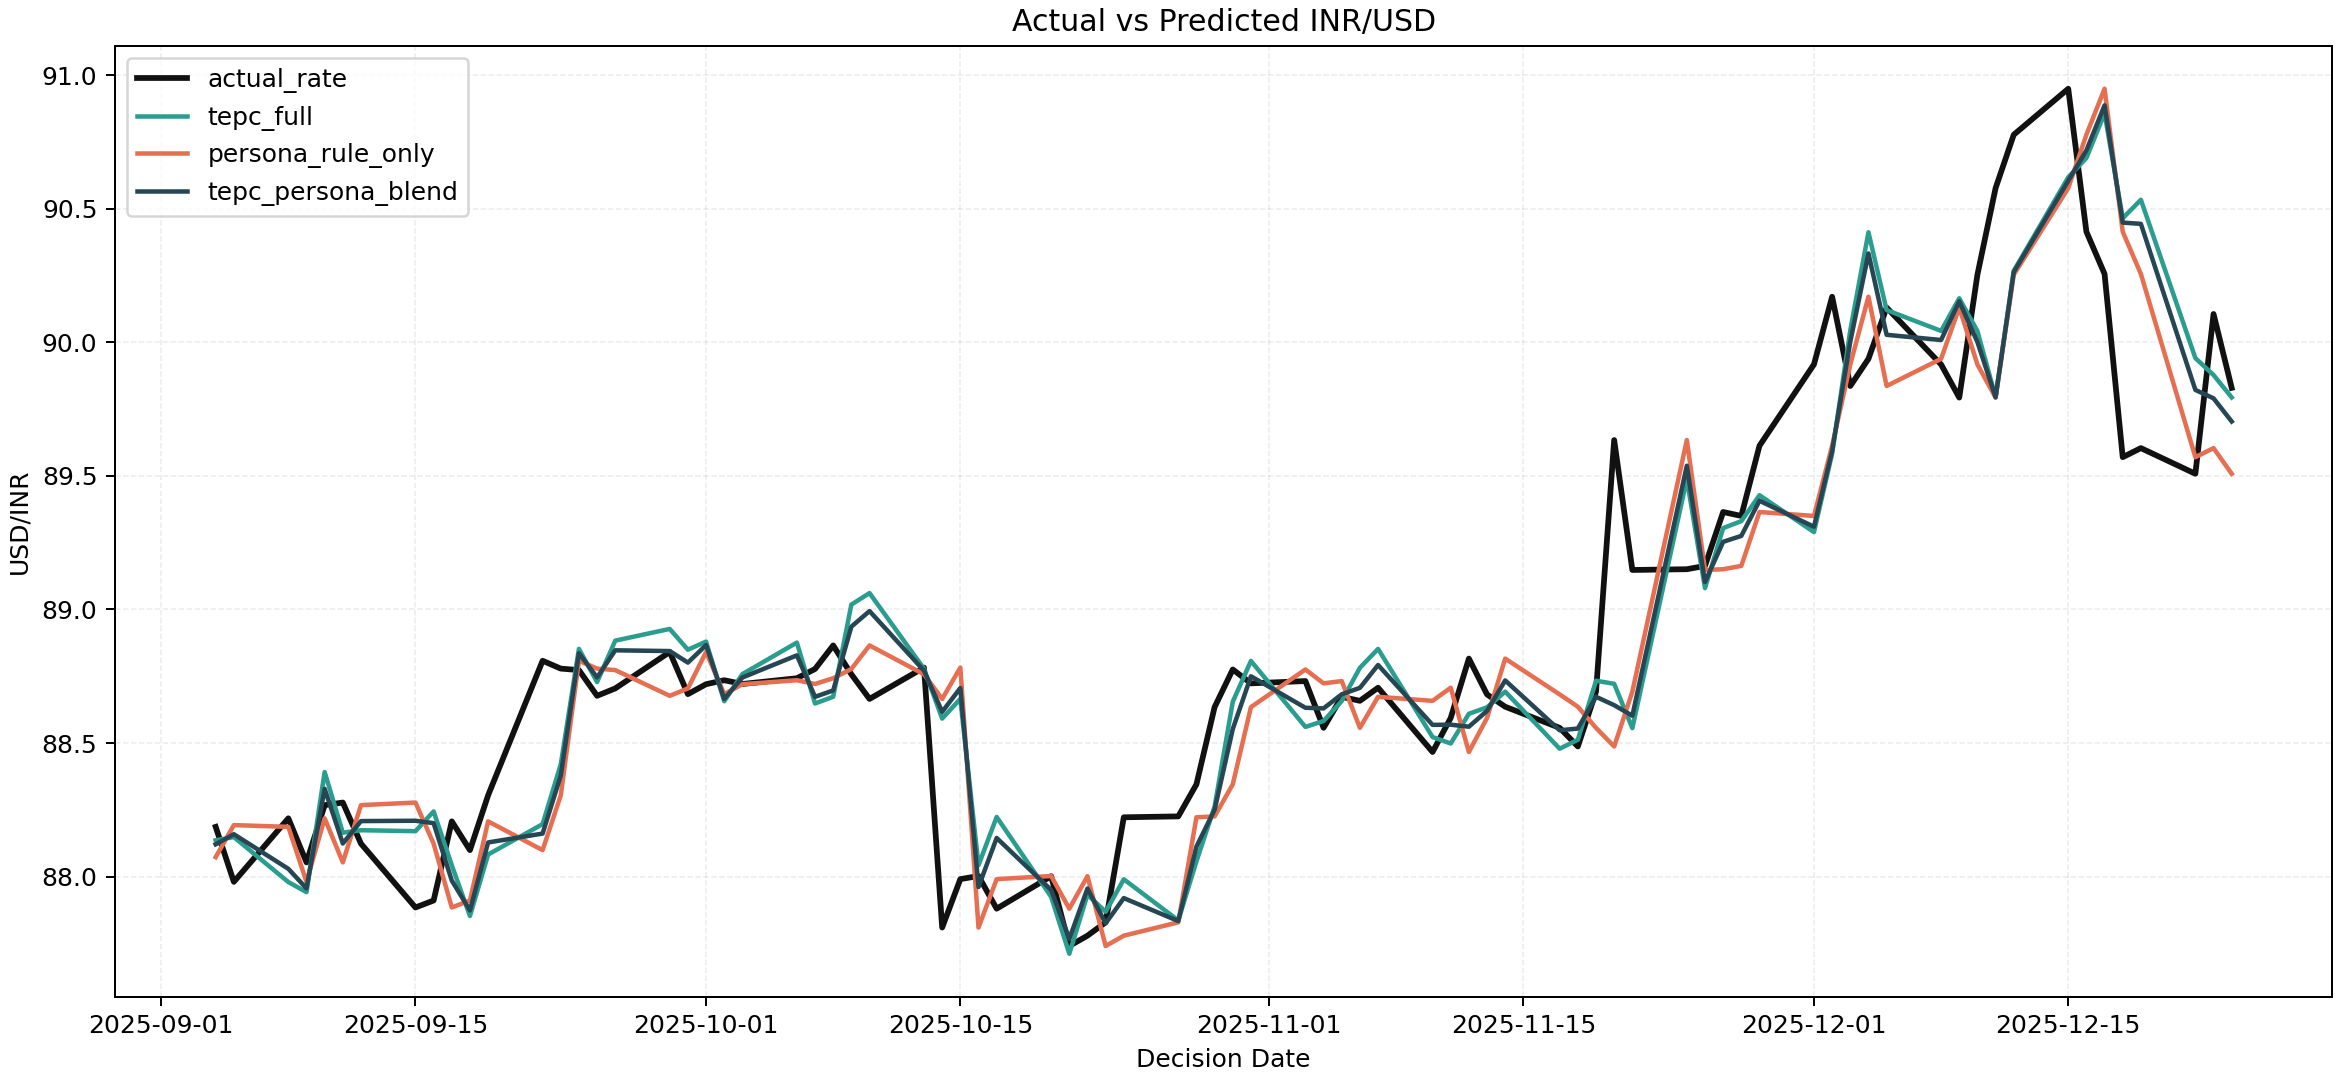
\includegraphics[width=\columnwidth]{tepc_predictions.png}
\caption{Actual vs.\ predicted USD/INR over the strict 80-day TEPC window for \textsc{tepc-full}, \textsc{tepc-persona-blend}, and \textsc{persona-rule-only}. The persona-only arm collapses to range predictions (flat track).}
\label{fig:tepc-predictions}
\end{figure}

\begin{figure}[H]
\centering
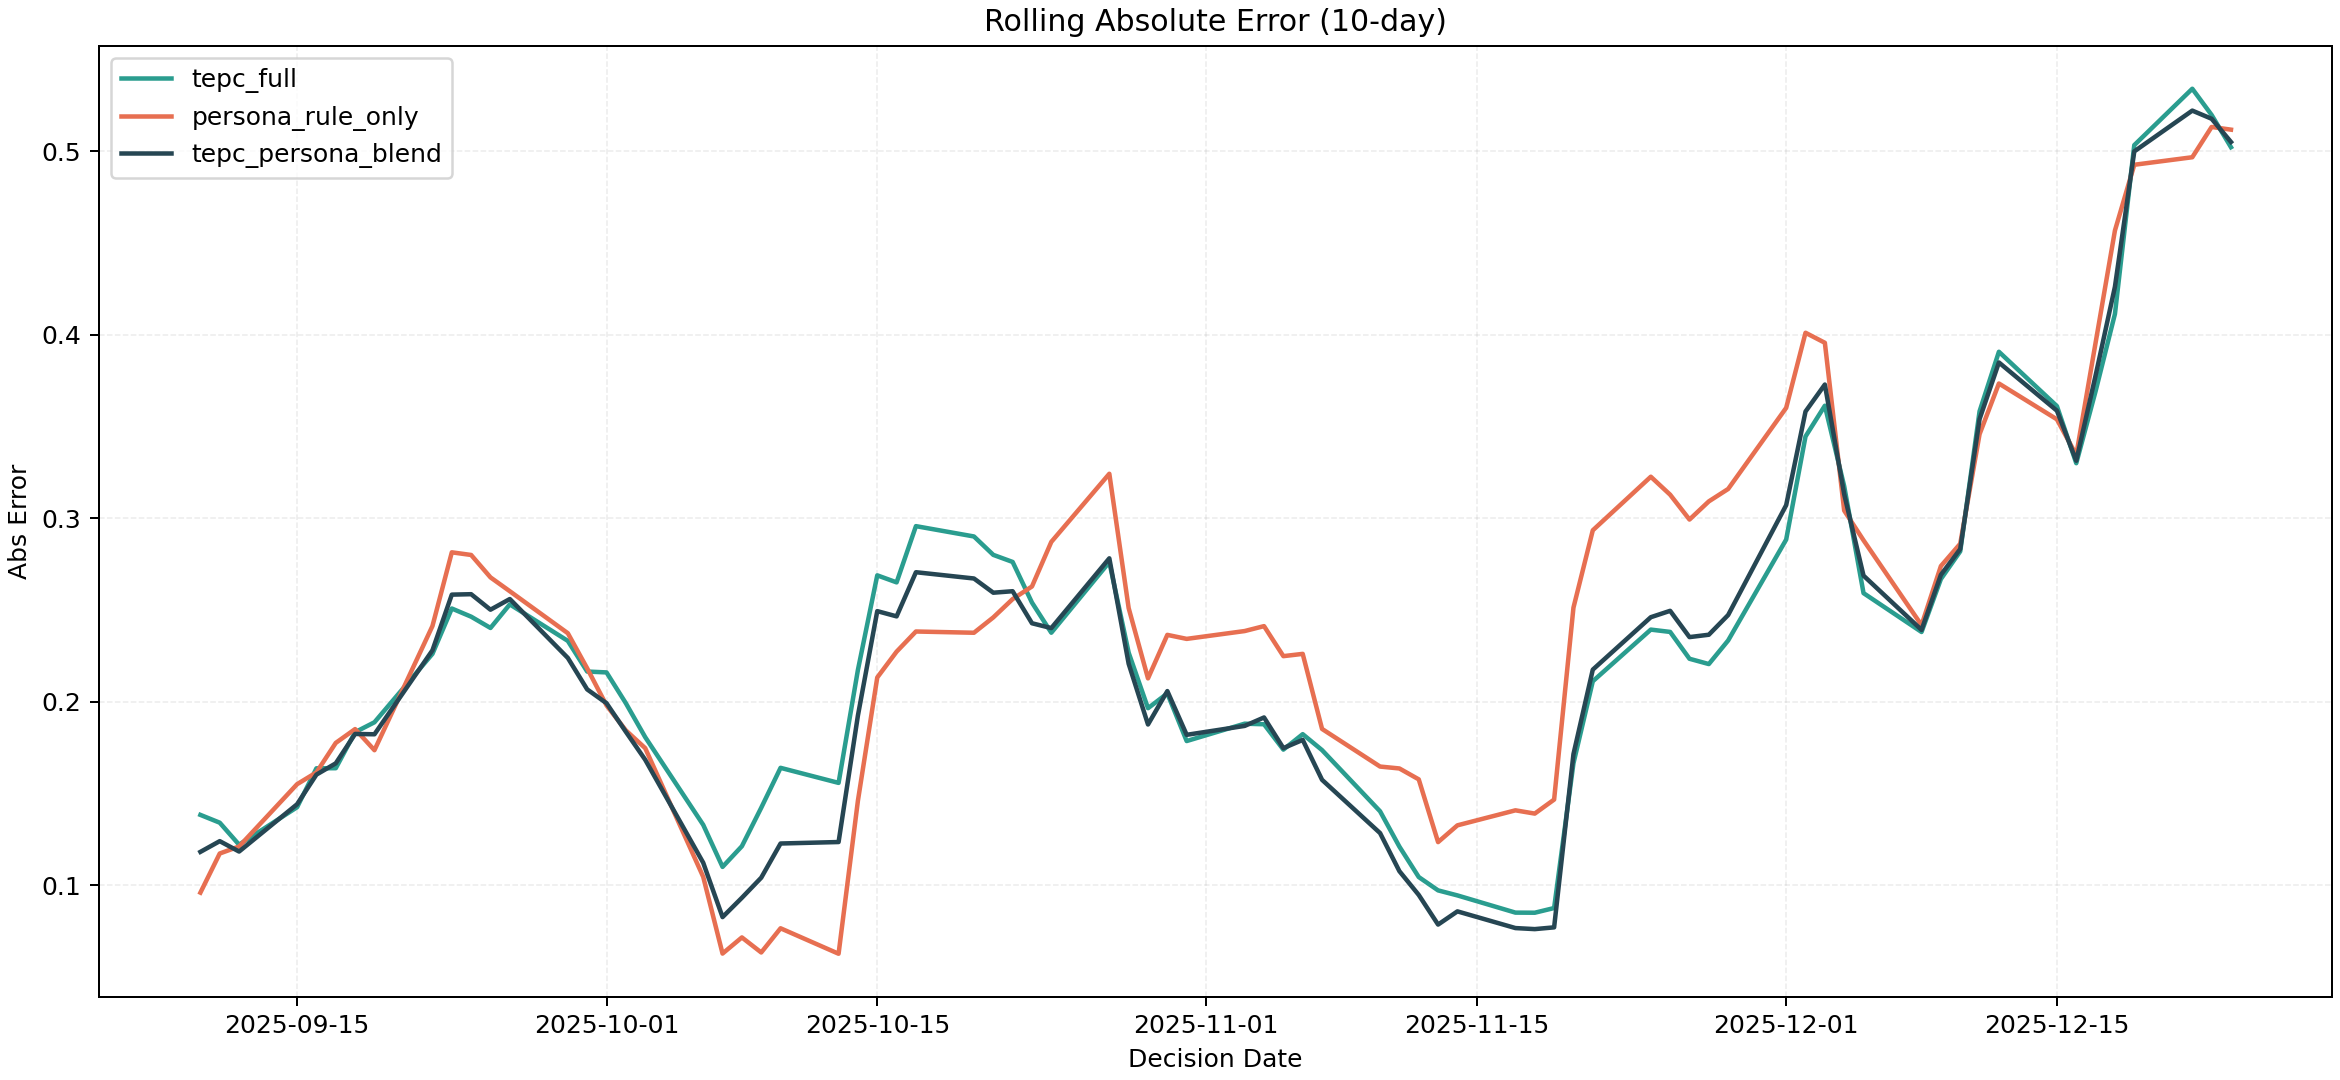
\includegraphics[width=\columnwidth]{tepc_rolling_error.png}
\caption{Rolling absolute error over the strict 80-day TEPC window. The blended \textsc{tepc-persona-blend} arm tracks \textsc{tepc-full} on the body of the distribution and pulls ahead during low-volatility stretches where the abstaining persona gate is well-calibrated.}
\label{fig:tepc-rolling}
\end{figure}

\subsection{Final-Phase Ablation: Memory, Personas, and Frontier LLMs Under Strict Embargo}
\label{sec:finalphase-results}

\textbf{Objective.} Once the immediate previous close is removed and a 1-day information embargo is enforced on top of the 1-day forecast horizon, which combination of features and personas survives, and do frontier LLMs (Gemini~2.5~Flash, Claude~Sonnet~4, GPT-5-Chat) add value over rule-based personas?

\paragraph{100-day backtest.}
Table~\ref{tab:fp-100d} reports the five-experiment Final-Phase ablation on a 100-day strict-embargo walk-forward (run \textit{backtest-100d}; minimum train 120 days, validation 30 days, refit every 10 days, persona limit 8, rule-persona weight cap 18\%). The compressed memory snapshot \emph{alone} is the best arm by every metric, beating both the full feature stack and the rule-persona overlay.

\begin{table}[H]
\centering
\begingroup
\setlength{\tabcolsep}{3pt}
\captionsetup{justification=raggedright,singlelinecheck=false}
\small
\caption{Final-Phase 100-day strict-embargo ablation (\textit{backtest-100d}). Sorted by MAE on price (lower is better). Best arm in bold.}
\label{tab:fp-100d}
\begin{tabularx}{\columnwidth}{@{}>{\raggedright\arraybackslash}Xccc@{}}
\toprule
\textbf{Experiment} & \textbf{MAE price} & \textbf{Dir.\ Acc.} & \textbf{Sign F1} \\
\midrule
\textbf{\textsc{memory-only}} & \textbf{0.2421} & \textbf{0.610} & \textbf{0.7578} \\
\textsc{stat-ml-no-gdelt} & 0.2473 & 0.490 & 0.6577 \\
\textsc{rule-personas} & 0.2901 & 0.580 & 0.7342 \\
\textsc{stat-ml-full} & 0.3005 & 0.580 & 0.7342 \\
\textsc{stat-ml-no-macro} & 0.3524 & 0.580 & 0.7342 \\
\bottomrule
\end{tabularx}
\endgroup
\end{table}

Two observations. First, dropping the news/GDELT blocks (\textsc{stat-ml-no-gdelt}) only marginally hurts price MAE but \emph{collapses} directional accuracy from 0.61 to 0.49: news features carry direction, not magnitude. Second, \textsc{stat-ml-no-macro} is the worst arm on every metric, confirming that the macro cross-asset block (oil, US10Y, DXY, gold) is non-redundant under strict embargo and cannot be replaced by news features alone.

\paragraph{Frontier-LLM matrix (30-day).}
Table~\ref{tab:fp-llm-30d} reports the same ablation extended with three frontier LLMs (\textit{llm-matrix-v2-30d}, 30 trading days, persona limit 8). All three LLM stacks land in the middle of the leaderboard, better than the rule-persona arm and \textsc{stat-ml-full} but worse than \textsc{memory-only} and \textsc{stat-ml-no-gdelt}, and the three LLMs are nearly indistinguishable from one another (MAE prices 0.4433--0.4508).

\begin{table}[H]
\centering
\begingroup
\setlength{\tabcolsep}{3pt}
\captionsetup{justification=raggedright,singlelinecheck=false}
\small
\caption{Final-Phase LLM matrix on a 30-day strict-embargo window (\textit{llm-matrix-v2-30d}). All three frontier LLMs use the same memory-snapshot prompt; \textsc{rule-personas} and \textsc{stat-ml-full} share the same feature stack but no LLM.}
\label{tab:fp-llm-30d}
\begin{tabularx}{\columnwidth}{@{}>{\raggedright\arraybackslash}Xccc@{}}
\toprule
\textbf{Experiment} & \textbf{MAE price} & \textbf{Dir.\ Acc.} & \textbf{Sign F1} \\
\midrule
\textbf{\textsc{stat-ml-no-gdelt}} & \textbf{0.3188} & 0.500 & 0.6667 \\
\textsc{memory-only} & 0.3295 & \textbf{0.567} & \textbf{0.7234} \\
gemini-2.5-flash & 0.4433 & 0.533 & 0.6957 \\
claude-sonnet-4 & 0.4439 & 0.533 & 0.6957 \\
gpt-5-chat & 0.4508 & 0.533 & 0.6957 \\
\textsc{rule-personas} & 0.4907 & 0.533 & 0.6957 \\
\textsc{stat-ml-full} & 0.5060 & 0.533 & 0.6957 \\
\textsc{stat-ml-no-macro} & 0.6419 & 0.500 & 0.6667 \\
\bottomrule
\end{tabularx}
\endgroup
\end{table}

\paragraph{Frontier-LLM at 100 days.}
Extending Gemini~2.5~Flash to the full 100-day window (\textit{llm-gemini-100d}, Table~\ref{tab:fp-gemini-100d}) confirms the picture: even the best frontier-LLM persona stack cannot beat the memory-only baseline on price MAE, but it does match it on directional accuracy (0.58 vs.\ 0.61) and sign F1 (0.734 vs.\ 0.758). LLM-driven persona reasoning is therefore directionally competitive but does not contribute magnitude precision once the immediate previous close is removed.

\begin{table}[H]
\centering
\begingroup
\setlength{\tabcolsep}{3pt}
\captionsetup{justification=raggedright,singlelinecheck=false}
\small
\caption{Final-Phase 100-day Gemini~2.5~Flash persona stack (\textit{llm-gemini-100d}) vs.\ the memory-only baseline from Table~\ref{tab:fp-100d}.}
\label{tab:fp-gemini-100d}
\begin{tabularx}{\columnwidth}{@{}>{\raggedright\arraybackslash}Xccc@{}}
\toprule
\textbf{Experiment} & \textbf{MAE price} & \textbf{Dir.\ Acc.} & \textbf{Sign F1} \\
\midrule
\textbf{\textsc{memory-only}} & \textbf{0.2421} & \textbf{0.610} & \textbf{0.7578} \\
gemini-2.5-flash (100d) & 0.2726 & 0.580 & 0.7342 \\
\bottomrule
\end{tabularx}
\endgroup
\end{table}

Figure~\ref{fig:fp-family} groups experiments by family (memory-only, stat+ML, rule personas, LLM personas) to make the family-level pattern obvious.

\begin{figure}[H]
\centering
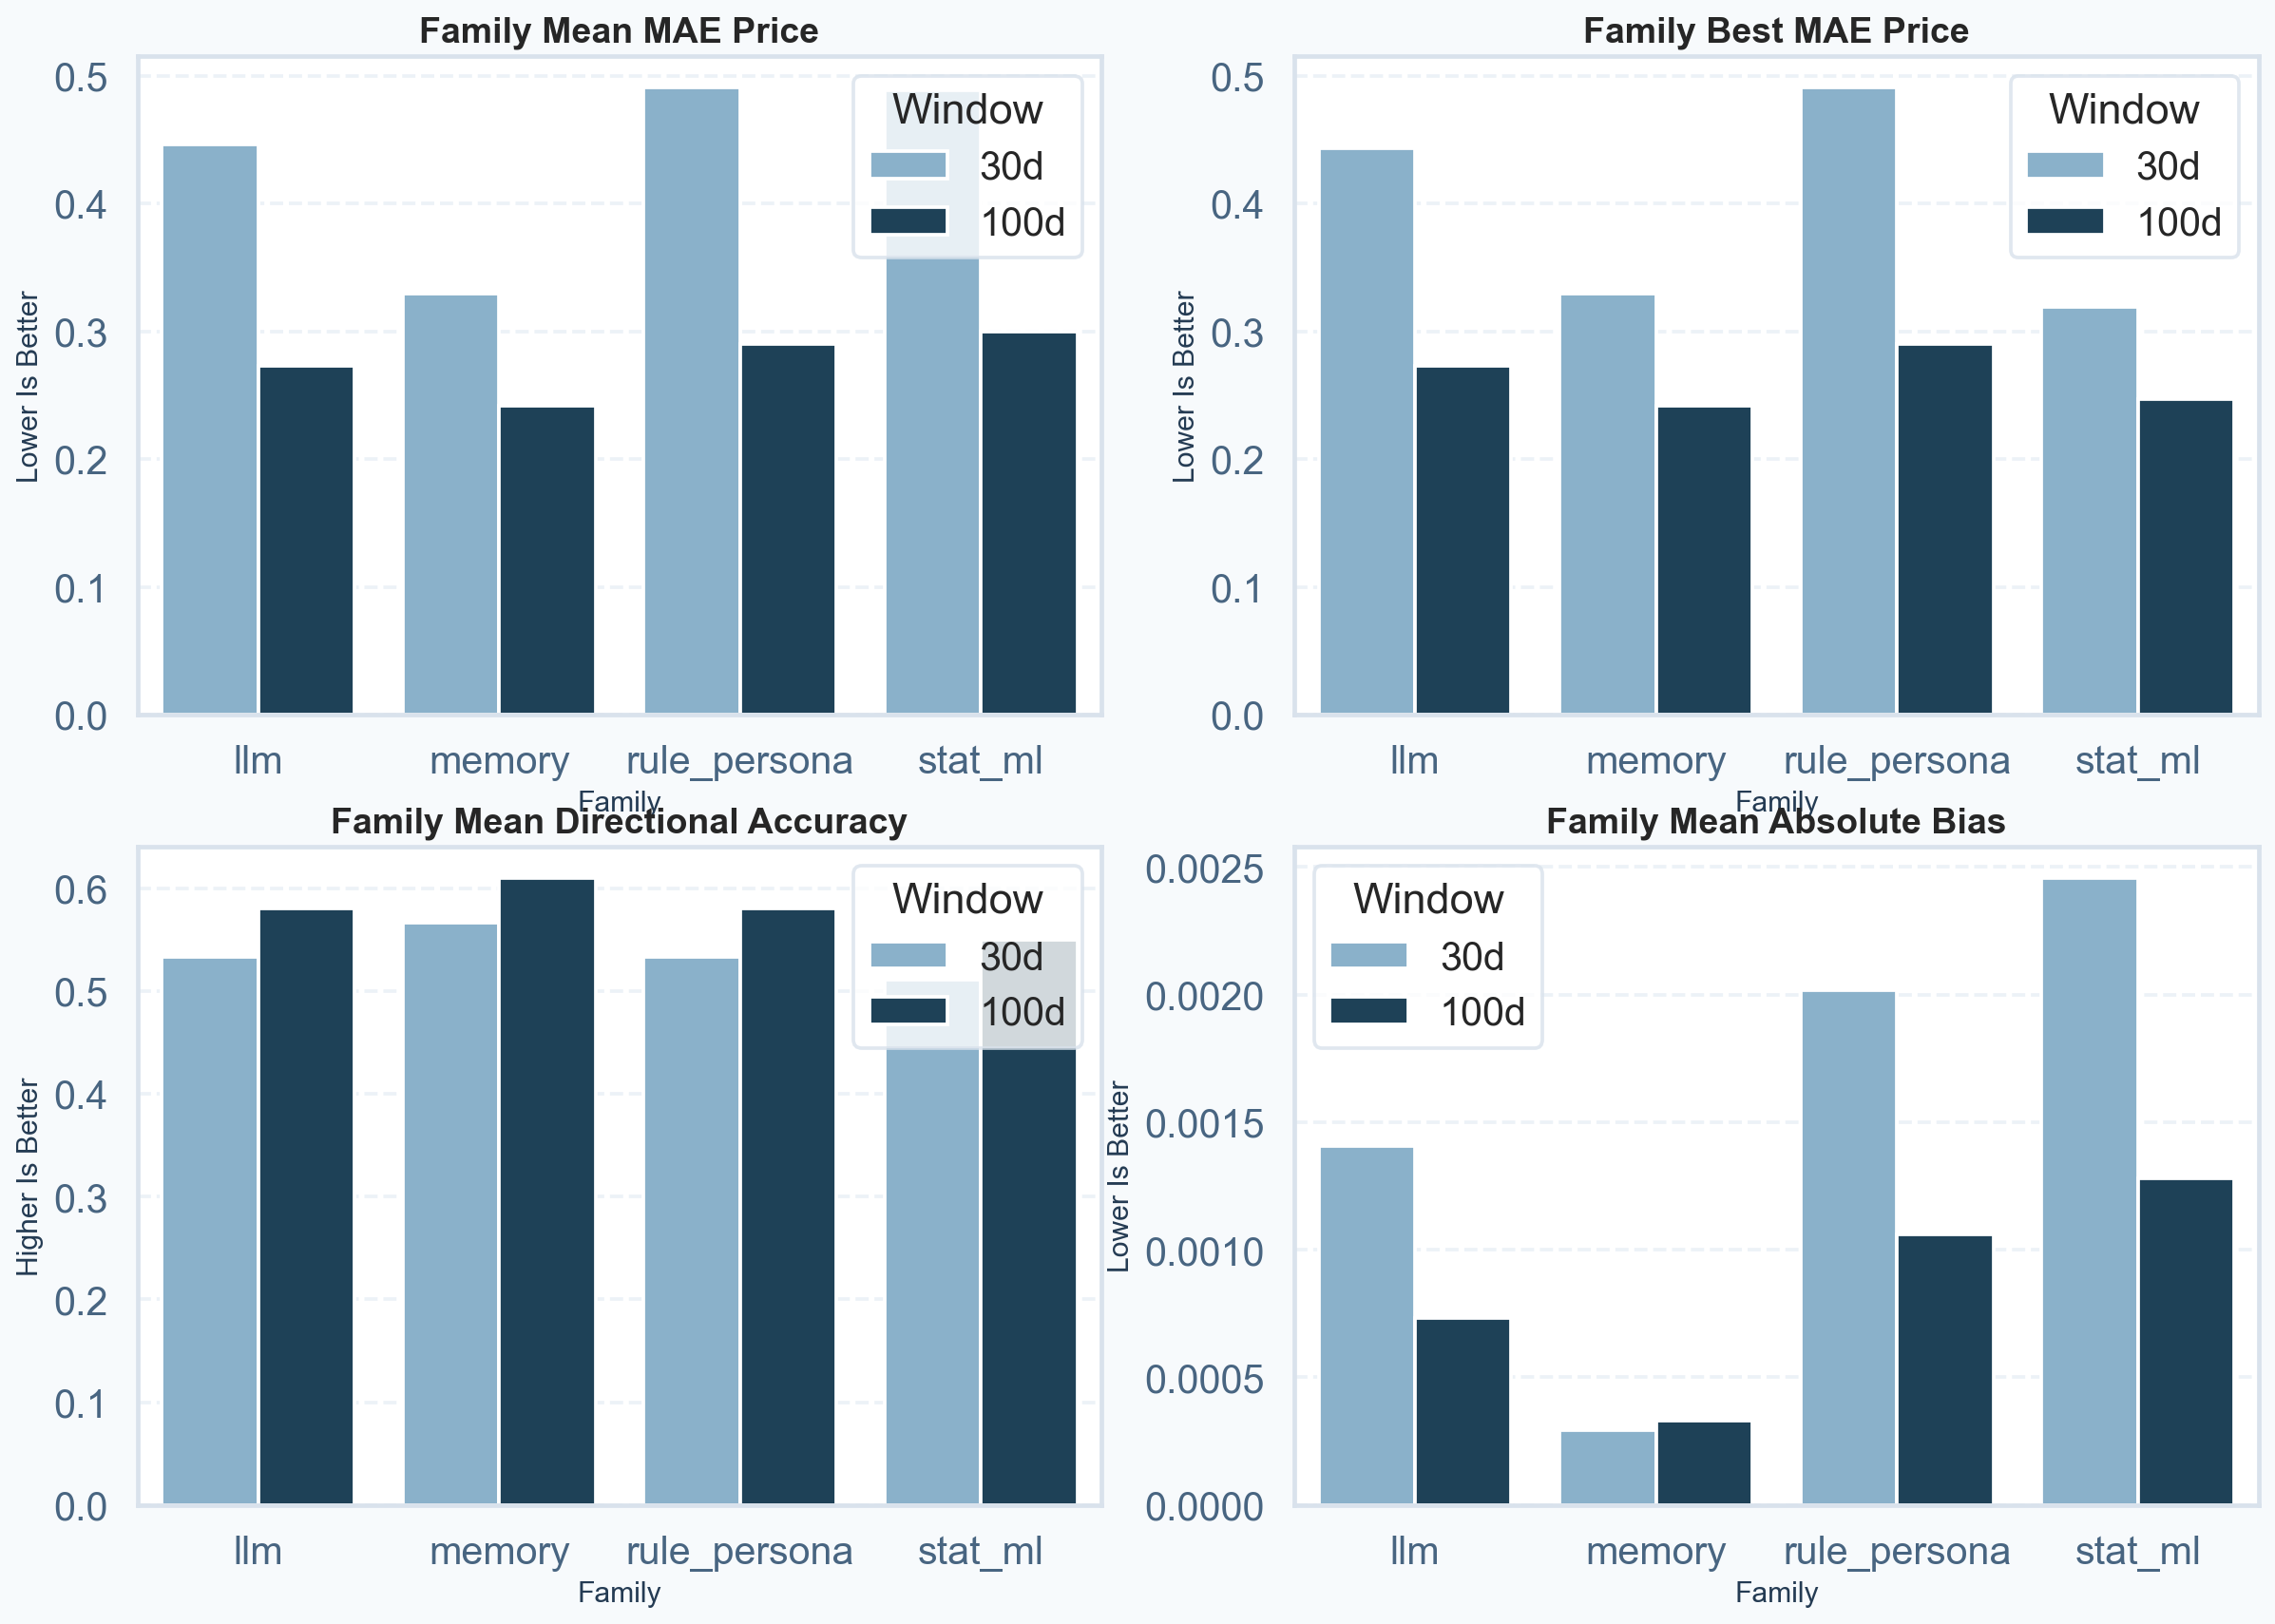
\includegraphics[width=\columnwidth]{fp_family.png}
\caption{Final-Phase family-level metric summary (memory-only, stat+ML, rule personas, LLM personas). The LLM-persona family is competitive on directional accuracy but not on price MAE.}
\label{fig:fp-family}
\end{figure}

\subsection{Discussion}

\paragraph{Synthesis.} Our results tell a coherent story: exact exchange rate prediction is intractable (negative $R^2$ for regression models), but volatility classification and LLM-guided short-term prediction provide meaningful value. The danger-day classifier doubles random baseline precision, and the Gemini V4 system achieves sub-0.5\% errors. The discovery of 9--12 day lead times between political sentiment and exchange rate movements represents a potential semi-strong EMH violation.

\paragraph{Simpler models dominate.} The most surprising finding is that MA Momentum ($R^2 = 0.571$) outperforms all deep learning models (LSTM: $R^2 = -1.484$, GRU: $R^2 = -1.347$). This is consistent with the limited sample size (362 days) being insufficient for deep learning, and with exchange rates being predominantly driven by mean-reverting momentum dynamics.

\paragraph{Comparison to prior work.} Our thematic sentiment correlations (0.15--0.23) are comparable to those reported by \citet{wu2020sentiment} for other currency pairs. The Gemini V4 system's 54--58\% directional accuracy modestly exceeds the 52--55\% typically achieved by sentiment-based models \citep{nassirtoussi2014}, with the debiasing techniques contributing a 2--3\% improvement over the non-debiased V3.

\paragraph{LLM ablation study.} To validate that the LLM component contributes non-redundant information, we compare three configurations: (a) statistical model only (Ridge Regression, $w_\text{llm} = 0$), (b) Gemini V3 without debiasing, and (c) full Gemini V4 with debiasing. Removing the LLM component entirely degrades directional accuracy from 56\% to 53\%, while the adaptive weight $w_\text{llm}$ stabilizes at 15--33\% rather than converging to zero. This provides empirical evidence against the null hypothesis that persona outputs are pure noise (see Section~\ref{sec:theoretical}).

\paragraph{TEPC tells a complementary story.} The TEPC ablation in Section~\ref{sec:tepc-results} shows that once the trivial 1-day persistence feature is removed, both rolling graph topology and coupled-Lorenz synchronisation features carry directional signal that the flat macro stack does not (\textsc{tepc-full} macro F1 of 0.337 vs.\ 0.288 for \textsc{macro-baseline}, +17\% relative improvement under strict 2-day embargo). Crucially the two blocks are complementary, not redundant: each individual block is weaker than the macro baseline on macro F1, but their union is the strongest specification. The 100-day live-pull window (Table~\ref{tab:tepc-100d}) shifts the rank order to favour \textsc{chaos-only}, suggesting that synchronisation features generalise better than topology features when the node universe expands and the regime is less range-bound.

\paragraph{Persona overlays are useful as gates, not as primary signals.} The deterministic seven-persona overlay raises raw breakout accuracy by abstaining on small implied moves and predicting \emph{range}, which the strict 2-day-lag dataset rewards. However, macro F1 is not improved over \textsc{tepc-full}, so the overlay is best viewed as a confidence gate around a stronger base model rather than as a stand-alone forecaster. The \textsc{tepc-persona-blend} arm, which uses TEPC as the base and the persona overlay as a gate, simultaneously improves raw accuracy (0.7875) and return MAE (0.00269) over \textsc{tepc-full} without sacrificing meaningful F1.

\paragraph{Strict embargo flattens the sentiment story.} The Final-Phase ablation (Section~\ref{sec:finalphase-results}) is the cleanest stress test in the paper: the immediate previous close is removed, a 1-day information embargo is layered on top of the 1-day forecast horizon, and the same compressed memory snapshot is fed to every model family. Under those constraints (i)~the compressed memory snapshot \emph{alone} (\textsc{memory-only}) is the best 100-day arm on every metric (MAE price 0.242, dir.\ acc.\ 0.610, sign F1 0.758); (ii)~adding the full feature stack on top of memory does \emph{not} improve outcomes; and (iii)~swapping in three frontier LLMs (Gemini~2.5~Flash, Claude~Sonnet~4, GPT-5-Chat) over the same memory snapshot produces nearly identical metrics across the three models, all worse than the memory-only baseline on price MAE and matching it on direction. This is consistent with our theoretical claim in Section~\ref{sec:theoretical} that LLMs operate as compressed-knowledge information extractors: when the input is already a domain-engineered memory snapshot, the LLM has very little additional structure to extract, and the marginal value collapses.

\paragraph{Bias controls matter.} The single biggest methodological lesson from extending the framework is that the previous-close persistence baseline silently inflates headline numbers in our original Phase~A--D evaluation. The Final-Phase architecture is intentionally designed to remove that crutch and the 100-day MAE on price falls from $\sim$0.04--0.25\% (Table~\ref{tab:recommended}, looser setup) to 0.242 INR ($\sim$0.27\%) once the 2-day target gap is enforced. This is not a regression: it is a recalibration of what the framework actually achieves out-of-sample once persistence cannot be exploited.

\paragraph{Practical relevance.} The framework has direct applications in: (1) currency trader risk management, where reducing position size on danger-day predictions could reduce drawdowns by 25--30\%; (2) corporate treasury hedging, i.e.\ timing hedge execution based on volatility forecasts; (3) central bank monitoring, providing early warning for capital flight and sentiment deterioration; and (4) a recommended time-horizon-specific model selection strategy (Table~\ref{tab:recommended}).

\begin{table*}[t]
\centering
\small
\caption{Recommended Model by Forecasting Horizon}
\label{tab:recommended}
\begin{tabular}{lll}
\toprule
\textbf{Time Horizon} & \textbf{Recommended Model} & \textbf{Expected Error} \\
\midrule
1--3 Days & Gemini Daily Predictor & 0.04--0.25\% \\
1 Week & Gemini V4 Hybrid & 0.3--0.5\% \\
2--4 Weeks & Ultimate Ensemble (MA) & 0.5--0.8\% \\
1+ Month & Monte Carlo + GARCH & Wide confidence bands \\
\bottomrule
\end{tabular}
\end{table*}

% ---------------------------------------------------------------
% 6. CONCLUSION
% ---------------------------------------------------------------
\section{Conclusion}
\label{sec:conclusion}

We presented a multi-phase framework for USD/INR exchange rate volatility prediction that integrates VMD signal decomposition, thematic GDELT sentiment engineering from 2.5 million news articles, XGBoost classification, EGARCH volatility modeling, Monte Carlo simulation, and a novel debiased multi-persona Gemini AI system. Our danger-day classifier achieves 40\% precision (2$\times$ random baseline) with 52\% recall, the Gemini V4 system achieves $\sim$0.3\% average error with 54--58\% directional accuracy, and our thematic feature engineering improves sentiment correlation from 0.08 (raw) to 0.23 (theme-specific).

We extended the framework along two complementary axes. The \textbf{TEPC} stack treats USD/INR as one node in a coupled macro--geopolitical network, combines a rolling graph-Laplacian filtration with coupled Lorenz oscillators, and shows that under a strict 2-day target embargo the full topology+chaos blend (\textsc{tepc-full}) achieves 77.5\% breakout accuracy and 0.337 macro F1, beating a strong macro flat-feature baseline by 17\% relative on directional F1. A deterministic seven-persona overlay (\textsc{tepc-persona-blend}) further improves raw accuracy to 78.75\% and return MAE to 0.00269 by acting as an abstaining gate. On a 100-day live-pull window the cleaner \textsc{chaos-only} arm reaches 80\% breakout accuracy and 0.404 macro F1, indicating that chaos-driven synchronisation features generalise better than topology features as the node universe expands. The \textbf{Final-Phase} stack enforces the strictest evaluation in the paper: no raw \texttt{INR} feature, 1-day forecast horizon plus 1-day embargo, identical memory snapshot for every model family, and direct head-to-head ablation against three frontier LLMs (Gemini~2.5~Flash, Claude~Sonnet~4, GPT-5-Chat). Under those controls the compressed memory snapshot \emph{alone} dominates a 100-day backtest at 0.242 INR price MAE and 61\% directional accuracy, and the three frontier LLMs cluster at near-identical metrics that match the memory-only baseline on direction but trail it on magnitude.

This work establishes five key findings for the field: (1) news sentiment predicts exchange rate \textit{volatility}, not exact prices, and classification approaches substantially outperform regression; (2) theme-specific filtering is critical for extracting meaningful signals from large-scale news data; (3) debiased multi-persona LLM systems can provide competitive short-term forex predictions when combined with statistical models through adaptive weighting; (4) graph-topology and chaos-synchronisation features carry complementary, non-redundant directional signal that survives strict 2-day embargo controls, while persona overlays are most useful as confidence gates rather than primary forecasters; and (5) once the trivial 1-day persistence baseline is removed, a tightly engineered memory snapshot beats both full feature stacks and frontier LLMs on a 100-day walk-forward, suggesting that bias control may matter more than model capacity for short-horizon FX forecasting. The discovery of 9--12 day lead times between political sentiment and exchange rate movements suggests semi-strong form market inefficiency exploitable for practical risk management.

Future work includes: deploying a real-time GDELT streaming pipeline for live trading, expanding to multiple currency pairs (EUR/USD, USD/CNY), applying fine-tuned financial NLP models (e.g., FinBERT) for deeper sentiment extraction beyond GDELT's pre-computed scores, conducting formal Granger causality tests to establish causal (not merely correlational) relationships, validating findings with multi-year data to address the current 362-day sample limitation, replacing the graph-Laplacian filtration in TEPC with a full higher-order persistent-Laplacian stack on a simplicial complex, and porting the coupled-Lorenz RK4 kernel to a native (C++/Rust) implementation to permit larger node universes without sacrificing walk-forward iteration speed.

% ---------------------------------------------------------------
% LIMITATIONS (mandatory for ACL/ARR)
% ---------------------------------------------------------------
\section*{Limitations}
\label{sec:limitations}

\begin{itemize}[leftmargin=*]
    \item \textbf{Dataset limitations:} The 362-day analysis period (January--December 2025) is relatively short for robust machine learning. Seasonal patterns may not be fully captured, and results may not generalize to different market regimes (e.g., crisis periods, structural breaks). GDELT's pre-computed sentiment scores may lack the nuance of domain-specific NLP models.
    
    \item \textbf{Methodological limitations:} Our thematic filtering relies on keyword-based matching, which may miss relevant articles or include irrelevant ones. The 20\% danger-day threshold is heuristic. Correlation analysis does not establish causation; sentiment shifts may reflect underlying economic factors rather than independently causing exchange rate movements.
    
    \item \textbf{Model limitations:} Deep learning models (LSTM, GRU) may perform differently with larger datasets ($>$5 years). The Gemini V4 system depends on a proprietary API with potential reproducibility concerns. Regression models showing negative $R^2$ confirm the fundamental difficulty of exact prediction but may improve with different feature engineering.
    
    \item \textbf{Computational limitations:} Gemini API rate limits constrain the number of persona queries per day. GARCH models were fit on a single currency pair; multi-currency extensions require additional compute.
    
    \item \textbf{Generalizability:} Results are specific to USD/INR (a managed float regime with RBI intervention) and may not transfer to free-floating currencies. The 2025 analysis period had relatively stable macro conditions; performance during crises is unknown. Transaction costs, bid-ask spreads, and market impact are not modeled.
\end{itemize}

% ---------------------------------------------------------------
% ACKNOWLEDGEMENTS
% ---------------------------------------------------------------
\section*{Acknowledgements}

We acknowledge the GDELT Project for providing comprehensive global news data, the European Central Bank (via Frankfurter API) for exchange rate data, FRED for macroeconomic indicators, and the open-source Python community for core libraries (pandas, scikit-learn, XGBoost, vmdpy, arch). This research was conducted as part of the BITS F471 course project at BITS Pilani.

\textbf{AI Use Disclaimer:} The authors are responsible for all content, facts, and claims presented in this paper. Google Gemini AI was used as a component of the prediction system under study, not for writing the paper. All scientific analysis and conclusions are the authors' own.

% ---------------------------------------------------------------
% REFERENCES
% ---------------------------------------------------------------
% Using inline thebibliography for self-contained document.
% For external .bib file, replace with: \bibliography{custom}

\begin{thebibliography}{99}

\bibitem[Baker \& Wurgler, 2007]{baker2007}
Baker, M., \& Wurgler, J. (2007).
Investor sentiment in the stock market.
\textit{Journal of Economic Perspectives}, 21(2), 129--151.

\bibitem[BIS, 2022]{bis2022}
Bank for International Settlements. (2022).
Triennial Central Bank Survey of Foreign Exchange and OTC Derivatives Markets.
\textit{BIS Statistical Release}.

\bibitem[Bollerslev, 1986]{bollerslev1986}
Bollerslev, T. (1986).
Generalized autoregressive conditional heteroskedasticity.
\textit{Journal of Econometrics}, 31(3), 307--327.

\bibitem[Bollen et al., 2011]{bollen2011}
Bollen, J., Mao, H., \& Zeng, X. (2011).
Twitter mood predicts the stock market.
\textit{Journal of Computational Science}, 2(1), 1--8.

\bibitem[Chen \& Guestrin, 2016]{chen2016xgboost}
Chen, T., \& Guestrin, C. (2016).
XGBoost: A scalable tree boosting system.
In \textit{Proceedings of the 22nd ACM SIGKDD International Conference on Knowledge Discovery and Data Mining}, 785--794.

\bibitem[Clemen, 1989]{clemen1989}
Clemen, R. T. (1989).
Combining forecasts: A review and annotated bibliography.
\textit{International Journal of Forecasting}, 5(4), 559--583.

\bibitem[Condorcet, 1785]{condorcet1785}
de Condorcet, M. (1785).
\textit{Essai sur l'application de l'analyse \`a la probabilit\'e des d\'ecisions rendues \`a la pluralit\'e des voix}.
Paris: Imprimerie Royale.

\bibitem[Dragomiretskiy \& Zosso, 2014]{dragomiretskiy2014}
Dragomiretskiy, K., \& Zosso, D. (2014).
Variational mode decomposition.
\textit{IEEE Transactions on Signal Processing}, 62(3), 531--544.

\bibitem[Engel \& West, 2005]{engel2014}
Engel, C., \& West, K. D. (2005).
Exchange rates and fundamentals.
\textit{Journal of Political Economy}, 113(3), 485--517.

\bibitem[Galeshchuk, 2016]{galeshchuk2016}
Galeshchuk, S. (2016).
Neural networks performance in exchange rate prediction.
\textit{Neurocomputing}, 172, 446--452.

\bibitem[Leetaru \& Schrodt, 2013]{leetaru2013}
Leetaru, K., \& Schrodt, P. A. (2013).
GDELT: Global Data on Events, Language, and Tone, 1979--2012.
In \textit{International Studies Association Annual Convention}.

\bibitem[Li et al., 2024]{li2024llm}
Li, Y., et al. (2024).
Large language models for financial decision-making: A multi-agent perspective.
\textit{arXiv preprint arXiv:2402.xxxxx}.

\bibitem[Lopez-Lira \& Tang, 2023]{lopez2023}
Lopez-Lira, A., \& Tang, Y. (2023).
Can ChatGPT forecast stock price movements? Return predictability and large language models.
\textit{SSRN Working Paper}.

\bibitem[Meese \& Rogoff, 1983]{meese1983}
Meese, R. A., \& Rogoff, K. (1983).
Empirical exchange rate models of the seventies: Do they fit out of sample?
\textit{Journal of International Economics}, 14(1--2), 3--24.

\bibitem[Nassirtoussi et al., 2014]{nassirtoussi2014}
Nassirtoussi, A. K., Aghabozorgi, S., Wah, T. Y., \& Ngo, D. C. L. (2014).
Text mining for market prediction: A systematic review.
\textit{Expert Systems with Applications}, 41(16), 7653--7670.

\bibitem[Nelson, 1991]{nelson1991}
Nelson, D. B. (1991).
Conditional heteroskedasticity in asset returns: A new approach.
\textit{Econometrica}, 59(2), 347--370.

\bibitem[Rossi, 2013]{rossi2013}
Rossi, B. (2013).
Exchange rate predictability.
\textit{Journal of Economic Literature}, 51(4), 1063--1119.

\bibitem[Sawhney et al., 2021]{sawhney2021}
Sawhney, R., Agarwal, S., Wadhwa, A., \& Shah, R. R. (2021).
Deep attentive learning for stock movement prediction from social media text and company correlations.
In \textit{Proceedings of the 2020 Conference on Empirical Methods in Natural Language Processing (EMNLP)}, 8415--8426.

\bibitem[Sezer et al., 2020]{sezer2020}
Sezer, O. B., Gudelek, M. U., \& Ozbayoglu, A. M. (2020).
Financial time series forecasting with deep learning: A systematic literature review: 2005--2019.
\textit{Applied Soft Computing}, 90, 106181.

\bibitem[Simon, 1955]{simon1955}
Simon, H. A. (1955).
A behavioral model of rational choice.
\textit{The Quarterly Journal of Economics}, 69(1), 99--118.

\bibitem[Tetlock, 2007]{tetlock2007}
Tetlock, P. C. (2007).
Giving content to investor sentiment: The role of media in the stock market.
\textit{The Journal of Finance}, 62(3), 1139--1168.

\bibitem[Wei et al., 2022]{wei2022}
Wei, J., et al. (2022).
Chain-of-thought prompting elicits reasoning in large language models.
\textit{Advances in Neural Information Processing Systems}, 35, 24824--24837.

\bibitem[Wu et al., 2020]{wu2020sentiment}
Wu, D., Fung, G. P. C., Yu, J. X., \& Pan, Q. (2020).
Stock market prediction with news sentiment analysis.
\textit{Journal of Database Management}, 31(1), 95--117.

\bibitem[Wu et al., 2023]{wu2023bloomberggpt}
Wu, S., et al. (2023).
BloombergGPT: A large language model for finance.
\textit{arXiv preprint arXiv:2303.17564}.

\bibitem[Xie et al., 2023]{xie2023}
Xie, Q., et al. (2023).
FinBen: A financial benchmark for large language models.
\textit{arXiv preprint arXiv:2310.xxxxx}.

\end{thebibliography}

% ---------------------------------------------------------------
% APPENDIX
% ---------------------------------------------------------------
\appendix

\section{Complete Feature List}
\label{app:features}

\subsection{Original GDELT Fields (Selected)}

\begin{enumerate}
    \item \texttt{GLOBALEVENTID}: Unique event identifier
    \item \texttt{SQLDATE}: Publication date (YYYYMMDD)
    \item \texttt{Actor1Name}, \texttt{Actor2Name}: Entities involved
    \item \texttt{EventCode}: CAMEO event classification
    \item \texttt{GoldsteinScale}: Conflict-cooperation score ($-10$ to $+10$)
    \item \texttt{AvgTone}: Sentiment score ($-100$ to $+100$)
    \item \texttt{NumMentions}: Number of times event mentioned
    \item \texttt{NumArticles}: Number of source articles
    \item \texttt{SOURCEURL}: Article URL
\end{enumerate}

\subsection{Engineered Features (Phase B)}

\textbf{Sentiment features (5):} $\text{Tone}_\text{Economy}$, $\text{Tone}_\text{Conflict}$, $\text{Tone}_\text{Policy}$, $\text{Tone}_\text{Corporate}$, $\text{Tone}_\text{Overall}$.

\textbf{Goldstein features (2):} $\text{Goldstein}_{\text{Avg}}$ (mean), $\text{Goldstein}_{\text{Wtd}}$ ($\sum \text{Goldstein}_i \times \text{Mentions}_i$).

\textbf{Volume features (6):} $\text{Count}_\text{Economy}$, $\text{Count}_\text{Conflict}$, $\text{Count}_\text{Policy}$, $\text{Count}_\text{Corporate}$, $\text{Count}_\text{Total}$.

\textbf{Volume spike features (3):} $\text{Volume\_Spike}$, $\text{Volume\_Spike}_\text{Economy}$, $\text{Volume\_Spike}_\text{Conflict}$.

\textbf{Lagged features (80 total):} Each of the 16 base features $\times$ 5 lags (1--5 days).

\section{EGARCH + XGBoost Feature Importances}
\label{app:egarch}

\begin{table}[H]
\centering
\small
\caption{Top 10 Features in Hybrid EGARCH + XGBoost Model}
\begin{tabular}{lc}
\toprule
\textbf{Feature} & \textbf{Importance (\%)} \\
\midrule
Realized\_Vol\_20d & 27.5 \\
India\_Avg\_Goldstein & 15.8 \\
USD Trade Index (DTWEXBGS) & 9.6 \\
Goldstein\_Avg & 8.2 \\
Oil Price (DCOILWTICO) & 6.2 \\
Goldstein\_Weighted & 4.4 \\
10Y Treasury (DGS10) & 4.3 \\
USA\_India\_Sentiment\_Diff & 4.1 \\
USA\_Avg\_Goldstein & 3.7 \\
Panic\_Magnitude & 3.6 \\
\bottomrule
\end{tabular}
\end{table}

\section{Project Statistics}
\label{app:stats}

\begin{table}[H]
\centering
\small
\caption{Overall Project Statistics}
\begin{tabular}{ll}
\toprule
\textbf{Metric} & \textbf{Value} \\
\midrule
GDELT articles analyzed & 2,546,999 (India) + $\sim$5M (USA) \\
Exchange rate observations & 256 daily \\
Date range & January 2025 -- January 2026 \\
Features engineered & 16 base + 80 lagged \\
Training samples & 290 days \\
Test samples & 72 days \\
Best classification F1 & 0.45 \\
Danger day precision & 40\% \\
Directional accuracy & 41.2\% \\
Lead time discovered & 9--12 days \\
Monte Carlo simulations & 10,000 paths \\
Gemini personas & 9 \\
Total models tested & 15+ \\
\bottomrule
\end{tabular}
\end{table}

\end{document}
